\documentclass[10pt,a5paper]{book}
\usepackage[utf8]{inputenc}
\usepackage{amsmath}
\usepackage{amsfonts}
\usepackage{amssymb}
\usepackage{graphicx}
\title{Project Fjorgyn}
\author{Marcel Gietzmann-Sanders}
\begin{document}
\maketitle
\tableofcontents
\newpage
\chapter{Shorts}
These are a collection of short essays capturing various milestones in my thought processes around Project Fjorgyn that I found significant. 

\section{The Cycle of the Tide}
\subsection{A Personal Quandary}
First of all, I'd just like to express my amazement at human society. What humans have been able to build over the 45 odd millennia we've been recording ourselves is absolutely incredible. But as with anything else we create it's a work in progress. Climate change, mass extinctions, poverty, starvation, human rights issues, we have no lack of big problems to solve as we continue to move forwards and create better and better versions of ourselves. 

Unsurprisingly, (and I think I share this with most people) I would rather like to have a part in our collective betterment. I'd like to engage with these monumental problems we face as a society and help move the needle. So pan to me sitting behind a desk building software for an internet service provider and it's clear to see that there are some uncertainties and insecurities bubbling through my being, most of which boil down to a simple question - can't I be doing more? Shouldn't I be doing more?

My initial approach to this personal quandary was rather unimaginative. I figured that if I was going to be truly effective at helping solve one or more of these problems I had to become a professional at solving these problems. For my problem of choice - the protection of the marine biosphere - that meant becoming a marine biologist. So, just about a year ago now I signed up for an intro to marine biology class at a local university and started mapping out my transition away from the space of commercial software. 

\subsection{To Be An Enzyme}
Thing is, as I began to learn more about marine biology, conservation, and the other disciplines involved in protecting our biosphere, I noticed two very important things:
There were already so many amazing people, many of whom were far more intelligent than me, already working in these fields.
And yet, the majors breakthroughs in the field seemed to keep coming from the outside.
To illustrate the last point, take the example of the drones that are now used to explore, map, and monitor our oceans. While marine biologists and conservationists have, no doubt, had an important role in influencing this particular version of the technology, it has nonetheless been robotics engineers who have opened the door. Satellite data, machine learning, geographical information software, crowd sourcing apps, the list goes on and on. Everywhere I looked I found engineers opening the doors to the breakthroughs in the field. 

This is not of course to say that the engineers are responsible for the breakthroughs. Obviously without the biologists and conservations there to guide the application of the technology, none of this would've happened. Nonetheless the pattern did get me thinking and my mind soon drifted toward biochemistry.

We, and by we I mean living, breathing biological beings, should not be possible according to the rules of inorganic chemistry. The reactions that turn our food into motions and thoughts and experiences are incredibly improbable. There is this whole idea of the "activation energy" required to get a reaction going, and for the vast majority of our biochemical processes their activation energy is far to high to ever support life. It's as if there's a series of locked doors and on the other side is life itself. 

Well the keys to these door are catalysts. Catalysts (amongst other things) reduce that activation energy so substantially that they quite literally change the rules of chemistry. What was before an improbable reaction becomes common place and, boom, life is born.

To me this is not unlike the relationship between technology and the stewards of our world. While many conservationists, biologists, farmers, and other world stewards are far smarter than I am, and could, given the time and resources, open the doors to things like machine learning, automation, remote sensing, drones, and the like for themselves, the fact of the matter is that they are up to the gills in all the work required to be a steward - conservation planning, running research projects, writing papers, building networks, the list is extensive. As a result they often simply don't have the space to open those doors - the activation energy is just too high. But when an engineer comes by and creates the technology themselves, suddenly the catalyst is there a whole new world is opened up to those same stewards. 

Technology catalyses action. 
 
Furthermore, I love this concept of technology as a catalyst rather than a solution, because it puts the focus on using technology to empower people rather than just handing them a solution. Teach a person to fish, right? By catalyzing rather than solving it leaves the engineer free to work on new problems while simultaneously leaving behind a whole workforce of stewards who can adapt and develop the technology on their own. For me, a budding software engineer, this was a powerful realization. Yet I knew there was more, for I was already familiar with the power of catalysts - in how it applied to myself. 

\subsection{Compound Interest}
I have always found it quite amazing how technology is able to compound on itself. Each time someone builds a new tool, that same tool makes it easier to construct other new tools. This has the same accelerative effect as compound interest, famously quoted by Einstein as the most powerful force in the world. 

Yet, this accelerative effect does not come for free. Simply creating some new piece of technology does not allow it to become foundational for other breakthroughs. Technology only falls into this elevated category when it is created with the appropriate level of abstraction in mind to allow its reuse across many different problems. Tools, not solutions, can be used to build other tools. 

I bring this up largely because it suggests an interesting strategy for tackling technical problems. If one starts with the low hanging fruit with the intention of building tools and not just solutions, then with each problem solved a new catalyst is created and other, previously difficult, problems suddenly become low hanging fruit themselves. Beyond making each step far more manageable and producing value more immediately, it also means that over time previously impossible problems become doable. This then brings me to my second tenet:

Building toolsets catalyzes development itself.

\subsection{A Pot of Gold}
And then it hit me - manageable projects resulting in foundational tools that empower incredible work and generate equally incredible impact - this is the stuff of an engineer's dreams. I suddenly had a vision of students and professionals working side by side on projects that would make them drool all while churning out work that empowered our world's stewards to build a better world. The match was there, the question that remained was simply - how? 

The answer, I think, is rather simple. It begins with a person, like myself, finding a project or two to work on and beginning to work out how to catalyze action while building out toolsets. As that individual developer builds report and skill, they will find themselves with too many projects to do on their own. So they take those incredibly interesting problems and find some buddies willing to work with them. So the mentorship begins. But as they help their buddies get going, they'll be developing a new skill - how to be a good mentor. This too can be taught, and so once their colleagues find themselves overloaded with projects they too can be taught how to teach. It is at this point that the floodgates have been opened because the organization will now grow itself as each new member begins to draw in members themselves - a pyramid scheme of the greatest intensions. 

This is how this veritable pot of gold can be handed out amongst all the engineers who stand to gain so much from it - through the mentorship of new developers. Through such peer to peer development it seems to me that an empire can be built. And so we have our final tenet:

Empires are built upon shared opportunity and mentorship.

\subsection{A Blueprint}
Finally then I have an answer to the question - can't I do more? The answer is yes, and the three tenets illustrated above are one version of how. By building technology I can empower our world's stewards. By focusing on the low hanging fruit and creating tools I can accelerate the development of that technology. And by sharing the wealth and mentoring people into it I can help found an empire. It is a magnificent feedback loop of empowerment - a tide to raise all ships. And it is something I am certainly going to try. 

\begin{figure}[!htb]
\center{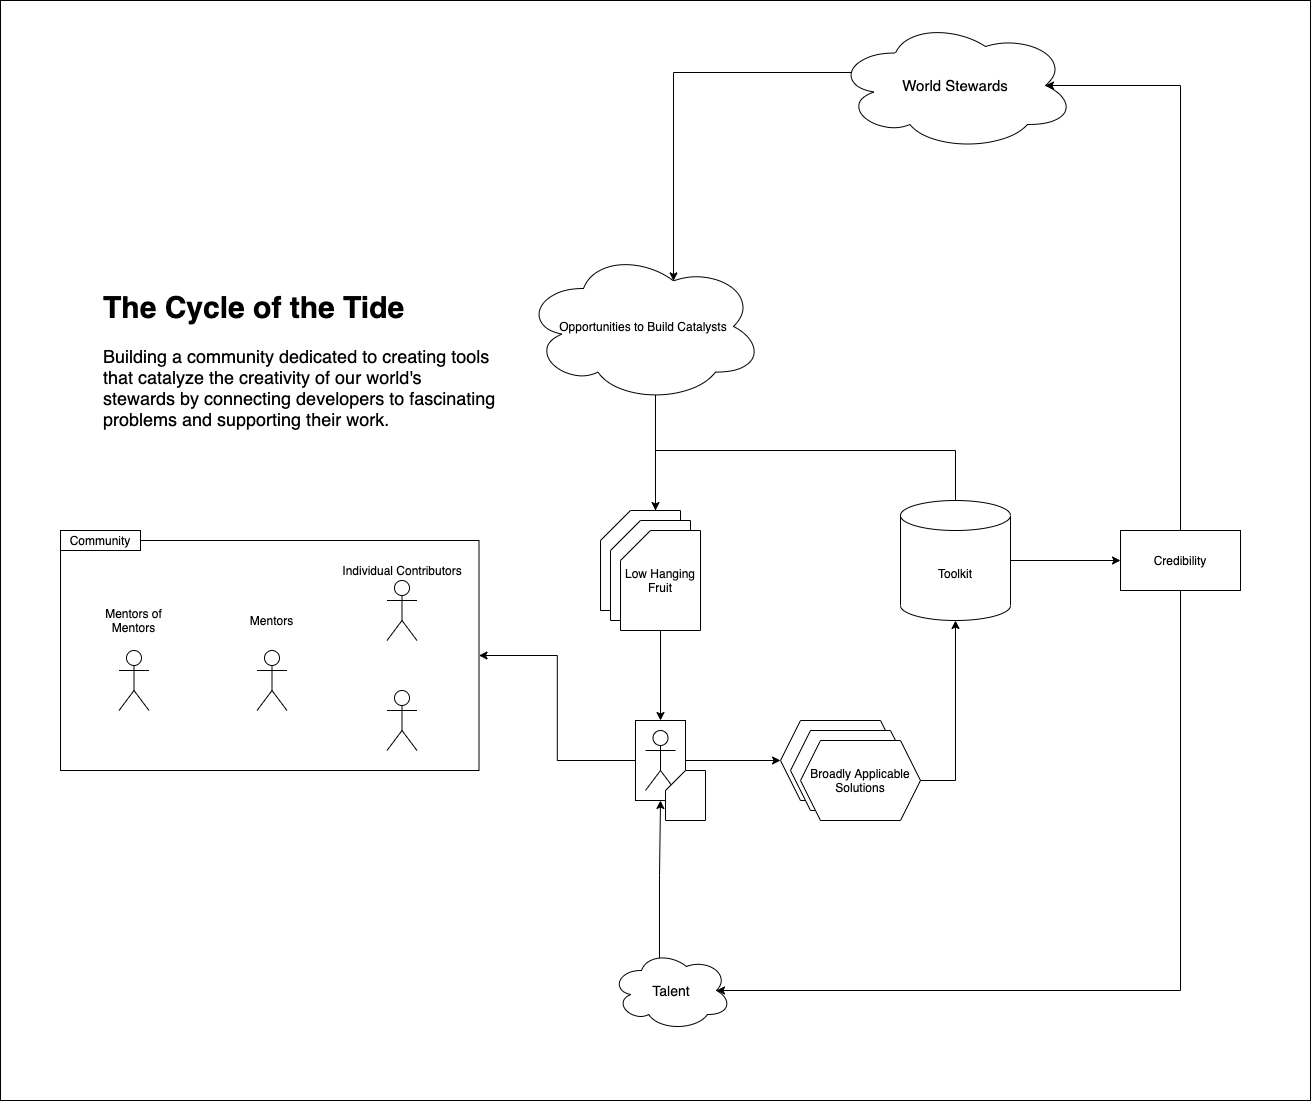
\includegraphics[width=\textwidth]
{figures/The_Cycle_of_the_Tide.png}}
\caption{\label{fig:my-label} The Cycle of the Tide}
\end{figure}

\textit{August 10, 2021}

\section{Cycles of Development}
So we have the Cycle of the Tide. Question now is how to actually execute that cycle. What are the conditions of success? How should we break up the projects into bite sized pieces? How should we work out prioritizations? What kinds of tracking should we put in place? Who are our stakeholders? How do we attract new talent? Yea, you get the idea - there's a lot of distance still left between our abstract set of goals and clear execution itself. 

To help us start covering this distance let us first recognize that there are essentially three components to the Tide Cycle - finding projects, executing on projects, and incorporating talent. In my mind the middle of those three is the axel around which the other two pivot, so in this post I'm going to do my best to lay the groundwork for execution. 

\subsection{Lifecycles}
Figuring out all the bits and bobs one has to pay attention to to manage a project is no small task. Thankfully there's a trick I've found very useful in the past - thinking about projects in terms of lifecycles. By being able to break a project into a lifecycle, we can focus on understanding each of the lifecycle components and how they relate to one another rather than trying to understand the whole all at once. Then once we've understood the details of each component we just add 'em up together to get the whole. So then, what is the lifecycle of a project?

\begin{figure}[!htb]
\center{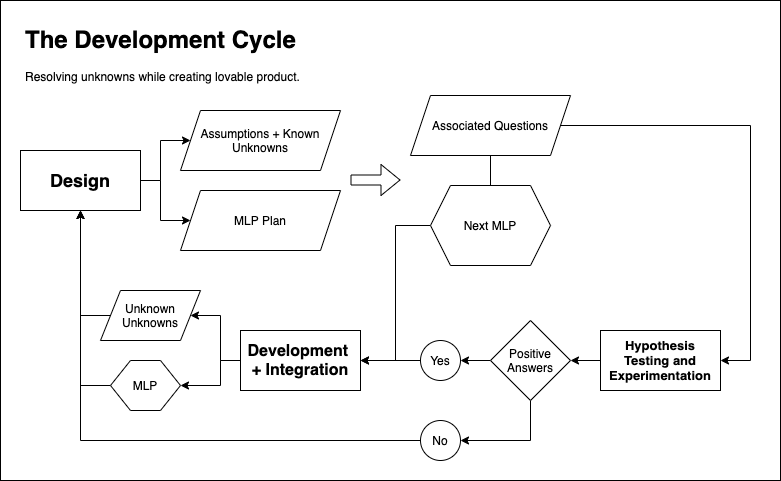
\includegraphics[width=\textwidth]
{figures/The_Development_Cycle.png}}
\caption{\label{fig:my-label} The Development Cycle}
\end{figure}


\subsection{Design}
All projects start in the same place - as an idea. At this stage there's a lot of unknowns. You don't necessarily have a perfect grasp of the problem or its context. You may not necessarily know exactly how what you're going to build is going to be used. You won't yet know all the tools you'll take advantage of or whether you've got the right resources in terms of data, compute and money. So it's important to dedicate a significant amount of time and energy to thinking and designing what's actually going to get built. That being said, it's easy to get lost in all the questions, so let's break it down. 

\subsubsection{What Are The Problems?}
This is the most critical question of all. Too often projects are built around solutions that someone dreamed up to a problem that same person barely understood. Given there are no lack of great articles on problem vs solution based thinking I won't go into detail here, but suffice it to say that you must ensure that you've framed your project in terms of a set of problems and not in terms of a set of solutions. 

\subsubsection{What's The Ecosystem?}
Answering this question is foundational to ensuring that what you build will actually get used. You have to understand the ecosystem your product is going to become a part of and how your product is going to get used. If you build an awesome GIS tool but then realize that it doesn't integrate with any of the tools the organization you're helping uses you're going to be really disappointed. Absolutely ensure that you understand how what you are going to be building is going to be used.

\subsubsection{How Will This Be Extended?}
Remember the purpose here is to catalyze action and building toolsets - not build finely tuned solutions. To truly catalyze action we must "teach a person to fish". If you build a model for someone that has to be retuned every time the data is updated, then you'd better make sure your users are able to do that tuning otherwise you won't have catalyzed anything. Therefore you have to spend time understanding how they will extend and update the tool so that you can build in the features required to make that doable for them. Self sufficiency has to be a goal here. 

\subsubsection{How To Make This Reusable}
An equally important goal is to ensure we're building toolsets that are reusable across a range of problems and not just solutions to a particular problem. Only by creating this kind of reusability can we ensure that we're accelerating our overall development across projects. This is an essential part of the Cycle of the Tide and therefore must be a priority in our brainstorming and design.

\subsubsection{Has This Been Done Before?}
A step often missed in the excitement of starting a new project is simply finding out if there are examples already out there to learn from. Take time to look at the body of work that already exists because anytime you can learn from someone else, the better.

\subsubsection{What Are The Possible Architectures?}
A solid architecture is essential. It's the tool you use to create a framework for good engineering practice. This is where you get to think about how best to modularize the work, how to take advantage of prebuilt tools, how to build good interfaces, how to test things well, etc. It's also where you'll start thinking about the problem end to end. Creating thorough possible architectures will save you a lot of time and pain in the long run.

\subsubsection{What Will We Use To Build It?}
Compute, data, tools, models - this is where we think about and enumerate our options for actually putting meat onto our architectural bones. No need to explain why this is important.

Now I expect you may be wondering - if we've just started this project, how on earth will we possibly have all the information required to answer these questions? For example what if we've just been asked to build a model and have yet to even understand what data sources we have available? Answer is, you don't have to be able to answer them all. The point of the design exercise is as much to discover the known unknowns as much as it is about actually answering questions. Indeed the result of your design work should never be a list of answers. Rather it should be a list of hypotheses and known unknowns. The hypotheses are questions you think you have the answer to while known unknowns are the ones for which you don't. This then is the real purpose of the design stage - to elucidate your assumptions and questions in a clear and well organized manner. Actually answering those questions and testing your assumptions is dealt with in the next stage of the lifecycle. But before we jump into that there's one last piece to the design stage we haven't addressed yet.

\subsubsection{How Will We Fail Fast?}
You'll notice that so far we've been working to discover our known assumptions and known unknowns. This should leave anyone who's managed a project before with a nervous question - what about the unknown assumptions and unknown unknowns? These are often the project killers. 

For example you'll have designed everything out beautifully, been building gorgeous modules and api's for months, only to discover that a tool you've used for ages has some edge case lack of support that you absolutely need thereby bringing your whole enterprise momentarily crashing down. Not a great feeling. 

Unknown assumptions and unknown unknowns are the mismatches and gaps between our mental theories of the world and the way the world actually works. Therefore the only way to find unknown unknowns is by integrating things into the real world. This means getting your tools used pronto. The faster you can get something into someone's hands (even if it's missing features or is just a mockup) the better because that means you're rooting out the unknown unknowns sooner rather than later. 

Therefore it's of the utmost importance that part of your design is a plan for getting products into people's hands as quickly as possible regardless of whether those products are complete, partial, or just mockups. I call each of these incremental products Minimal Lovable Products or MLPs. So beyond our enumeration of hypotheses and known unknowns, an MLP plan must also be a product of our design process.

With that last piece handled we can now move onto the next stage of a project's lifecycle - hypothesis testing and experimentation.

\subsection{Hypothesis Testing And Experimentation}
The actual descriptions of this stage and the next are actually quite short. That's because thanks to your thorough designing process, the whole program for the rest of your project is already set down! Now all that's required is going through and ticking off boxes. 

So what actually goes on during this stage of the project? Remember our main goal is to fail fast and iterate quickly so that we can uncover unknown unknowns effectively. Therefore this stage is all about getting to the point where we can build something to quickly get in people's hands - i.e. our next MLP. That being said we may also have some rather existential questions looming about that fall into the known unknowns category. We obviously want to deal with those as well. As such this stage can be broken into two parts:
\begin{enumerate}
\item Addressing the known unknowns and assumptions that threaten the feasibility of the project.
\item Addressing the known unknowns and assumptions needed to build our next MLP.
\end{enumerate}

Finally, this stage is not just about answering questions but also considering the ramifications the answers have on our design. As we tick off the questions and validate our assumptions we must also update and and expand the design to match. Therefore with each question we answer we must ask ourselves how they impact each of the sections of our design listed above. 

\subsection{Development}
We've finally made it to the point where we have enough information to build some kind of minimally lovable thing! The purposes of this stage are simple:
\begin{enumerate}
\item Build our minimally lovable product (remember it might be as simple as a mockup).
\item Get our MLP into the hands of some users.
\item Document what we created and how it was received.
\item Update the design with what we've found. (Use the questions from the design stage to guide the investigation)
\end{enumerate}

This will be where those unknown unknowns show their faces, so it's important that you stay on the lookout for them by asking whether anything about your original answers to the design questions have changed in light of what you've actually found to be the case. 

Also worth mentioning here again is that catalysis comes from self sufficiency so on thing to keep an eye out are cases where a tool requires extra features to allow for that self sufficiency. These should not be ignored.

\subsection{Again!}
At this point you've answered a lot of questions, validated assumptions, created an MLP, discovered some unknown unknowns, and just generally done a lot of work. Now what? Well now it's time to repeat. You'll have an updated design and a next generation MLP to pursue, so it's back to the hypothesis testing and experimentation needed in order to pave the way toward your next MLP.

Eventually, as you keep repeating this cycle, you'll end up with all your questions answered and a final product that's already comfortably in the hands of your users. And so the development cycle will be complete. 

\subsection{Keeping Track Of It All}
Alright that was a lot so let's summarize:
\begin{enumerate}
\item \textbf{Design}: Using the questions listed above as a guide, create a compendium of assumptions and questions as well as a plan for MLPs.
\item \textbf{Hypothesis Testing and Experimentation}: Answer any existential project questions and broach the hypotheses and questions needed to tackle the next MLP.
\item \textbf{Development}: Build the next MLP, put it to use, and observe the results.
\item \textbf{Repeat}: Onto the next MLP.
\end{enumerate}

With this lovely lifecycle in place I hope it's now clear how to track the development of a project. Each stage has clear goals that should be concrete enough to allow for setting expectations while the overall project can be tracked through the repeated cycle through each of the stages with updates to the overall design. To help illustrate this I've thrown together the following super basic templates.

\begin{figure}[!htb]
\center{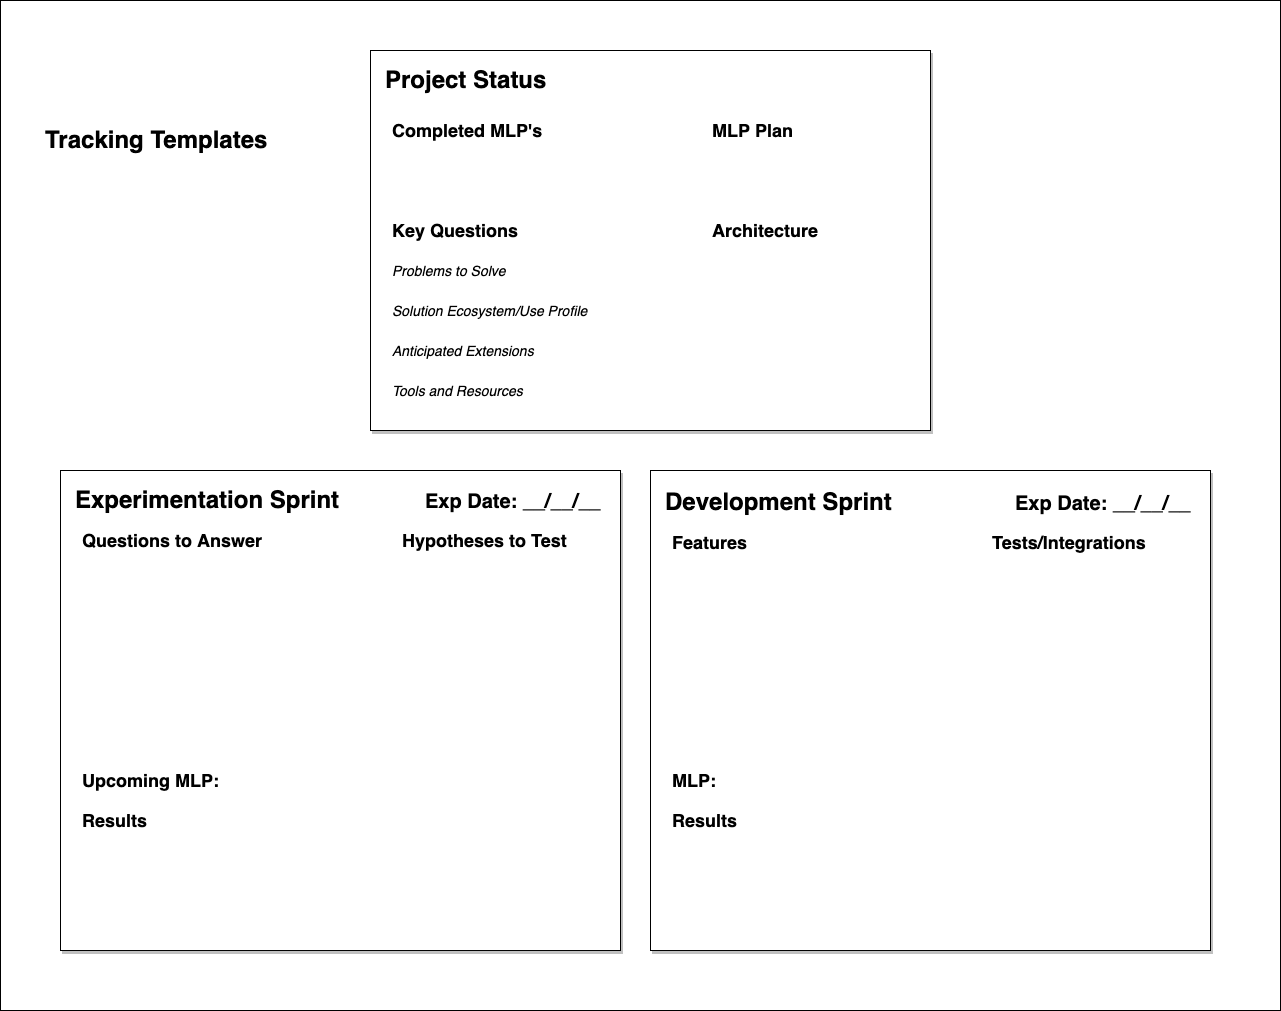
\includegraphics[width=\textwidth]
{figures/Tracking.png}}
\caption{\label{fig:my-label} Tracking it All}
\end{figure}

As you can see, the overall project state can be captured in one place while the history of the project is tracked by the various "sprint" cards built up over time. Altogether these capture everything from the roadmap, to the day to day tasks, to the project's record at meeting expectations while also capturing the results, learnings, and features found and built along the way. 

\subsection{The Development Cycle}
So there you have it - my take on the development cycle and how to keep track of it. Obviously there are plenty of other ways to manage projects out there, but I hope, at the very least, this perspective provides you with some useful food for thought. 


\textit{August 11, 2021}

\section{Delving Deeper - Everything but the How}
At this point we've discussed some of the various overarching questions present in the design of any project. But as you'll immediately realize if you start trying to answer those questions in earnest, those overarching questions are quite broad. Therefore, if we're really going to do a reasonable job covering and dealing with them we need to break them down a little bit further. 

Before we do that let's make a distinction between two kinds of question present in the design. I'll call them technical vs vision. The technical questions are all about how to get things done. Architecture and tools both fall into this category. Vision is all about the what, why, when, and where. Use cases, self sufficiency, overall problems, and so forth all fall into this one. In this post I'm going to dig deeper into the vision aspect, i.e. everything but the how. 

\subsection{Use Cases}
Obviously the very first question you must go about answering is - what are the problems I'm trying to solve - for as I said in a prior post there's a lot to be said for solving problems rather than creating solutions. That being said this particular brand of question is really only answered when you understand how people are going to use your tools so for me everything starts with use cases. 

Use cases are simply how people are going to be using the tools/technology that you build. For example if I were talking about building a new pizza oven I'd have to think about how people are going to assemble ingredients, put things in the oven, configure the oven, use it, and remove and enjoy the result. In other words the use cases are really user journeys. Because they are journeys we can use the same trick we used for product development as a whole and break the use cases into clearer elements by creating a lifecycle. These lifecycles will be composed of a series of stages and dependencies and for each of these we can ask the who, what, why, and when.

By building out a lifecycle for each use case (or user journey) and carefully thinking through each stage and dependency in those lifecycles, we will create a complete picture of the tool and its ecosystem. Each component becomes something to test and build and as we continue developing our product we can incrementally update the user lifecycles with any learnings we find along the way. Our progress in building the tools are then described by completing these lifecycles. 

Returning to the question of what problems are we trying to solve, we can look back through our lifecycles and understand the various issues we are solving in each stage or across stages. By doing things this way we ensure we capture details about how things get used in addition to what people are going to be getting at the end of the day. For example instead of just stating that our problem is "making a good pizza", by building out a lifecycle we might realize we also have the problems of "doing it easily" and "doing it configurably". 

So to summarize the first step to answering the vision questions is to create lifecycles for each use case; understand each stage/dependency in terms of who, what, why, and when; and then derive our overall problems from those lifecycles and stages. Keeping diagrams of these lifecycles is super useful for keeping track of the state of a project and incrementally adding in new learnings. 

\subsection{Teach a Person to Fish}
So we've captured how people are going to use the tools. But you'll recall that in order to ensure those tools act as catalysts we require self sufficiency on the part of the user. What does this mean? It means your tool had better be extendable. Extensions are thus the other half of the vision questions. 

We can start breaking up this large set of overarching questions by recognizing that there will be two kinds of technology that we're putting together - core technology and extensions. Core is going to be whatever's needed to allow for extensibility and extensions will be everything else. While this may seem like we're putting far too much into the extensions bucket remember that you'll want to start training users how to make extensions as quickly as possible so that their work can be catalyzed as quickly as possible. This is the only way we'll be able to find unknown unknowns in extendability with any expedience. 

Second we must recognize that just noting what kinds of extensions we expect doesn't necessarily mean those extensions are accessible. In order to truly catalyze work we need to make sure our technology's "energy barrier" to extension is suitably low enough. Therefore we're going to have to develop extension helpers. This can be as simple as documentation or as complex as a web tool - it totally depends on your users. 

Finally, people usually aren't going to teach themselves, so there needs to be a curriculum of sorts for teaching people how to make extensions and use the tools. 

To summarize, we have four components we're building: core, extensions, helpers, and curriculum. Now while we obviously need to document each of these in order to keep track of them you may question whether we should really be building extensions. Isn't that what the users are supposed to do? Well, often times, your users will still be learning how to use the tools and won't be up to the task of building extensions right off the bat. Yet, there may be extensions required to keep the project meaningful and moving forwards. Therefore your extensions are going to split into support and user developed. Support extensions are the ones you are building to keep the project moving forwards. Of course eventually you'll want all the extensions to be user developed, but while the project is under active development you'll want to keep track of both and methodically wean off of support extensions. 

The wonderful thing about breaking things up into these components is that we can answer and detail each of these pieces in turn and capture what needs to be accomplished separately for each. For example you can spend time just understanding what extensions need to be enabled, which need helpers, which are going to be support vs user developed and so on. Then, separately, you can think about what's going to be in your curriculum, where various users are in that curriculum, and how to move them forwards. And then you can turn to your core tech and work out designs and components for that separately. It just gives you a lot of small problems with clear bounds to solve instead of one overwhelming mass of vagueness. 

\subsection{Timelines}
Alright, so at this point we've got a whole lot of smaller, well defined components to think through that are going to each give us a whole slew of tasks to chase after. How on earth do we organize all these tasks into something coherent? Well that's where the MLP plan comes in. By taking all of these little tasks, organizing them into MLPs, and then planning the succession of MLPs, we take our smorgasbord of deliverables and create a neat, well organized timeline. And with that done, everything but the how is handled.

\subsection{Summary}
So let's summarize all of that. 
\begin{enumerate}
\item When dealing with our big overarching questions it's useful to divide the problem into technical questions and vision questions.
\item We can tackle the vision questions by considering use cases and extensions.
\item For use cases we can create use case lifecycles that break up into stages and dependencies. By subjecting each of those components to that questions of who, what, why, and where we can fill in the full set of lifecycles.
\item For extensions we can make a division into four categories of work: core, extensions, helpers, and curriculum. Extensions can be further divided into support and user developed. 
\item For each of the components we've now identified, we can dig in and understand what each means, what we know, what we don't, and what needs to be done. This work will result in a large number of tasks requiring organization.
\item This organization can be accomplished by taking all of those tasks and questions, organizing them into useful MLPs, and then organizing those MLPs into a timeline.
\item And finally, by capturing all of this in diagrams and notes, it'll be easy to keep track of everything that's going on while also allowing for incremental updates to the whole picture as we learn new things. 
So there you have it! One formula for dividing and conquering everything but the how. 
\end{enumerate}


\begin{figure}[!htb]
\center{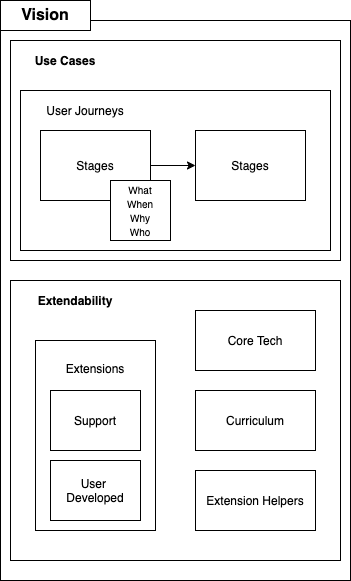
\includegraphics[width=\textwidth]
{figures/vision.png}}
\caption{\label{fig:my-label} Vision}
\end{figure}


\textit{August 22, 2021}

\newpage

\section{Servant Leadership}
Recently, as I've been thinking more and more about The Tide, I've been wondering about what makes for a good leader. I've occupied several small leadership roles in the past, but if the hope is, at some point in the future, to lead an organization, it seems prudent to figure out what made great leaders great. So I've been doing some reading and some thinking and there's a pattern that keeps cropping up. And it starts, as with many things that come out of my mind, with categories of action.

Broadly, I've noticed that there seems to be five things great leaders do. The first four are:
\begin{enumerate}
\item Energize - drum up motivation, excitement, and energy in the people around them
\item Actualize - open up the pathways to allow that energy and motivation to turn into action
\item Drive Coherence - find ways to create synergies between people's actions in order to achieve great things
\item Stem Incoherence - root out and expunge activities that would obstruct progress and synergy
\end{enumerate}

While certainly not comprehensive there's a kind of completeness to these four that I find lovely. It all begins with building up the energy and motivation required to take on the narrative any particular group might pursue. Great leaders have always been the kind of people who can stoke a fire in peoples' souls. While there is usually a nugget of that passion already present, it takes leadership to really light that tinder into something more. But once that fire has been stoked, without more fuel it will just burn out quickly. This then brings us to the second of the categories above - people need to have a means to actualize their energy. Good leaders have this laid out and ready to go. They don't leave people waiting but rather point them straight toward the gates. The best of leaders go even further and ensure that the path forward supplies all of the necessary ingredients for flow because they know that by creating manageably challenging work that provides people with a consistent cadence of success they'll be able to get the very best out of their followers and keep that fire stoked in their hearts. Sometimes this will include the training required to prepare people for the work. With these two categories of action they are able to stoke the fire within and then give it the fuel needed to burn steadily and consistently. As such, they create the individuals who, fundamentally, form the organization. 

With people active and playing their part, a good leader's attention then turns to ensuring that nothing their followers do is done in vain. Indeed they want to make sure that the work done has the greatest impact possible. This is where our last two categories come in - by nurturing coherence and weeding out incoherence a leader is able to weave the work of many individuals into a rich and meaningful fabric. In contrast to the first two categories which focused on the individual, these two focus on the health of the group as a whole. By keeping a healthy eye on both of these levels the leader can ensure that the organization continues to progress and grow. 

Now each of these four categories are really just a means to an end. So where is the end? Well, remember that I said that I've noticed five broad categories of action in great leadership. The fifth and final of these is narrative creation - great leaders craft a rich and meaningful narrative and it is this narrative that is the end to our means. I believe great leaders do this because they recognize two things:
\begin{enumerate}
\item Every other player in an organization has their hands full becoming an expert on their part to play and therefore must depend on someone else to become an expert on the whole.
\item They are the only ones receiving inputs from all parts of the organization and therefore are best placed to form drive consensus.
\end{enumerate}

Therefore great leaders realize that their followers depend on them for the narrative. This leaves leaders with a moral imperative to build and maintain the best narrative they can because people are staking no small part of themselves in that narrative. In much the same way that we depend vitally on farmers for food, those in the organization depend vitally on their leaders for the narrative that will ensure their work was not in vain. This, in my mind, places a requirement on the leader that they be a servant to their people and not the other way around. For how else can they ensure that they are looking out for the best interests of all those involved?

Indeed this servant leadership idea extends beyond just the creation of narrative. Think back to our four categories above. When energizing people, is it more effective to energize out of fear or belief? Obviously working to motivate people positively is going to be far more effective at creating meaningful, long term energy. What about actualization? As already mentioned, people do their best work when they feel like they can have sustainable flow. Burning people out, putting them in bad working conditions, these kinds of things are simply counterproductive. Even promoting coherence and stemming incoherence fall into this line of thought. By working to make the group as coherent as possible (both internally and externally) they are preventing disappointment, uplifting people, and generally providing an environment in which people can thrive. All in all, the best leaders do their utmost to make sure that they've built a world that uplifts the individuals within it. 

And indeed this is the best summarization of a great leader that I can think of - someone who works to build and actively grow an environment in which people can thrive by taking the role of servant leader. The narrative, the energizing, the actuation, the nurturing of synergies; all of these things are really just to serve the greater purpose of providing an opportunity for people to thrive and do great things. And that, at least to me, seems to jive pretty well with the whole spirit and intention of The Tide. 


\begin{figure}[!htb]
\center{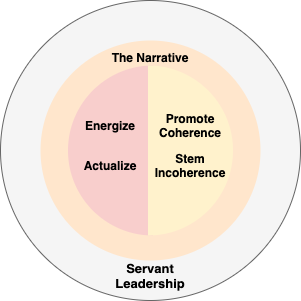
\includegraphics[width=\textwidth]
{figures/Leadership.png}}
\caption{\label{fig:my-label} Leadership}
\end{figure}

\textit{August 29, 2021}

\newpage

\section{Think, Then Code}
To me, as a developer, this is probably the most important rule of thumb there is:\linebreak

\textit{Before writing any code, design, design, design.}\linebreak

And yet, it's the kind of the advice that always seems to matter most when you want to follow it the least.

\subsection{Time Crunch}
We've all been here - your stakeholders are asking for something to happen in a period of time that's at least a little too small to be comfortable, and getting the work done is painted as an emergency. This is the likely the last place you're going to feel like taking the time to sit back and think things through carefully - you don't have the time or resources to spare for that! And yet, this is perhaps the most important time to do just that. 

There are many ways to stifle productivity. It might be a lack of monitoring that makes tracking down bugs (or even realizing they exist) near impossible. It might be scale issues that bring the development cycle to a standstill. It might be a plethora of bugs arising from misunderstandings about the system one is working with. The list goes on and on. But there are essentially two ways these issues are uncovered - either by thinking the problem through and creating a clear design, or by finding these things after building something. In the latter case you still end up having to go back and do the design, it's just that you only got there after doing a lot of throw away work. Obviously, when there's a time crunch, doing as little throw away work as possible is of the utmost importance. 

Now, even if you do throw together a design, it's often tempting during a time crunch, to put off worrying about design elements focused on longevity (things like scalability, extensibility, etc) because you feel like you just need to get something working now. Yet emergencies are rarely isolated events and usually end up extending across many, many different weeks as new features and products are required to truly dig a project out of the hole it finds itself in. Therefore ensuring that your productivity remains high over the long run is a much better strategy than trying to get through the current emergency by taking on technical debt that reduces productivity in the next one. You have a long road ahead of you - build for it. 

\subsection{When Everything's Easy Peasy}
The opposite situation is also one where it will be hard to follow the rule of think before you code. You know the situation - you're dealing with a problem you know so well you feel like nothing can really go wrong and you can just do everything on instinct. This assumption, is a hypothesis and just like in the case of the time crunch there are two ways you're going to test that hypothesis - by either thinking things through or by building something that may prove you wrong. For anyone who's done development, you'll know that no matter how well you think you know a problem, anytime you're doing something new there are little details that can quickly derail well intentioned plans. Therefore, once again, to avoid throw away work, just take the time to think things through carefully - otherwise you'll be setting expectations to your stakeholders that suddenly, out of hubris alone, you won't be able to meet. 

\subsection{When You Just Want to Get Your Hands Dirty}
Now you may ask, doesn't all of this fly in the face of the "fail fast" mentality? Not at all. Remember, a clear design, is more often going to be a series of questions that need to be answered than anything completely concrete. So even in the case where you're just wanting to find your unknown unknowns as rapidly as possible, taking the time to think things through carefully is important. If you don't, the "unknown unknowns" you discover may simply be answers to questions you could have answered at the outset with a little bit of thought, once again leaving you with unnecessary throw away work. Put another way, to guarantee that you're actually going to find things that lie outside of the scope of your understanding of the problem, you have to clarify your understanding of the problem first.

To summarize all of this, clear designs help you boost productivity, avoid unnecessary throw away work, and establish better expectations. In the end there are only two roads to discovering what's in your best interest - up front in thought or after you've built something you now want to get rid of. So, think first and then build something beautiful. And remember, the value of that thinking often scales proportionately with the pressure to skip skip it. 

\textit{September 13, 2021}

\section{Stewards and Weavers}
So far in discussing the tide we've focused on developing projects. This leaves an obvious and essential omission - how do we develop people? Given people are the center of any enterprise, helping them grow is of the utmost importance. 

Now obviously, I'm not about to solve "how to develop people" in one short blogpost, but I'd like to share something of a starting off point. We begin with the notion that central to personal development is understanding one's role both now and in the future. Without this kind of direction, we won't have a good sense of what we're trying to develop too. So what is the role held by those uplifting the tide? To get a sense of this we can start with those the tide seeks to help - stewards.

What is a steward? If we think in terms of means and ends, a steward is someone who focuses on a few ends and develops them through a plurality of means. For example an ecologist might use a variety of different tools - grant proposals, classes, research, software, etc. - to understand and protect a particular ecosystem. Many means, one end. From this point of view we can see just how essential stewards are, as if we're going to run something with any kind of expertise we will need stewards. 

But there's a problem, as stewards tend to silo. Restrained by the time and energy required to delve deeply into a particular end they have only so much time, energy, and resources to delve into the various means that are available to them. What's needed are people with deep external expertise who can weave a connection between them and these means. These weavers, as I'll call them, are the mirror of stewards. Whereas stewards apply a plurality of means to a few ends, weavers apply a few means to a plurality of ends. Together they form a complete web amongst the various disciplines. 

With that analogy of mirroring in mind it should be clear that weavers empower the tide. They are responsible for creating the connections that catalyze the work of stewards. This then is the role that we are trying to develop into as practitioners of the tide. Given weavers are practitioners of a few means to many ends we can also derive the main points of focus in development. Weavers must think carefully on the disciplines they wish to practice and then work towards mastery of those disciplines. This satisfies the depth of expertise in a few means. To satisfy the many ends component of being a weaver, weavers must also practice both being cognizant of many other fields and being good at identifying and pivoting to areas of impact within those fields. 

This then is our starting off point for personal development as a weaver. Identify what you wish to apply, work on mastering it, and learn how to spread your net wide and often. By developing these skills we can be assured of developing a stronger tide. 

\textit{September 24, 2021}

\section{Cartography}
\subsection{Maps and Layers}
If you've ever played around with maps (paper or digital) you'll have noticed that they change dramatically with the scale of area covered. If you're looking at a map that details a single city or town the detail will be so high as to point out individual museums, alley ways, and the like. If on the other hand you look at a map of a whole state, all of that detail will have disappeared to be replaced by the major routes, towns, and features of the state. There is obvious usefulness to this change in the level of abstraction. If you're trying to understand how to move throughout the state, any detail beyond the major routes and towns is just going to overwhelm and confuse you. But if a high level of detail is not present when you're navigating your destination, you'll never get where you're going. This property of maps provides a nice perspective for what I think is a general rule of human thought and organization. There is only so much detail we can think about at any one time without getting overwhelmed and losing the value of the information. Therefore the only way to organize extremely large systems is to create multiple layers of organization that build one on top of the next. 

The process for building these layers is relatively straightforward. Essentially you start by building a "map" at the highest level of resolution until you recognize that you've reached that "overwhelming limit". At this point you create a new layer of abstraction that allows you to break your full map into many individual maps with a layer on top to guide you through them. Then you keep building out your map with these layers until it becomes clear that your uppermost layer is once again too dense at which point you create a new layer on top of that and repeat. 

This hierarchy of layers is what allows us to organize any amount of detail and scope without blitzing our brains. It should also be noted that building a hierarchy of layers this way doesn't only help us build the map in the first place, but also makes it much easier to think about and update in the future. Rather than having to update or think about the whole space all at once, we can focus on one piece at a time. In summary, these layers allow us to tame the space and think effectively. 

Turning back to our catalysts we can already see that we've been doing this layering. Each of the questions we've outlined has represented a different "town" or "province" within the larger map of each catalyst. By building out a "map" for each of these we've been able to concentrate the full detail of each of our catalysts into manageable droplets while also providing detail on how they all connect. 

Yet as we build more and more successful tools, opportunities to combine our catalysts and build off of them will arise. You can think of this like individual hamlets and villages becoming aware of one another. No longer do maps of each town suffice - we now need a map of the whole continent. And so, a new layer arises. This new layer represents the ways in which catalysts connect and form entities far greater than the sum of their parts and thus ends up being a mapping of the full problem space in which the catalysts exist. Obviously this is a very important layer, so how do we go about building it?

\subsection{Drawing the Problem Space}
The whole point of this new layer of abstraction is to understand how our individual catalysts can connect into components larger than the sum of their parts. But before we can connect them we must know what we are trying to connect. This gives us our first step in drawing up this new layer of our map:\linebreak

Identify the catalysts and tools (not all will necessarily be built by you) that you're looking to connect and coordinate.\linebreak

With that done it's time to start making connections! At first blush this seems like a pretty vague and undirected activity, but I find that starting from the goals and working backwards really gets the creativity flowing. We can begin by collecting what we already know:\linebreak

Catalog the supported activities, intended catalyzations, expected extensions, and currently known use cases relevant to the tools and catalysts in question.\linebreak

Having the known goals laid out gives us an opportunity to consolidate. Are there overlaps between these various goals? Are some of these goals actually multiple sides of the same coin? Are there themes throughout that can be discovered and elaborated upon? Through this exercise we'll end up building a map of the problem space that is disentangled from and therefore elevated above the specificities of any one tool or catalyst - we're starting to a get a view of the bigger picture.\linebreak 

Consolidate the problem space into a map disentangled from and thus elevated above the individualities of each tool/catalyst. Get a sense of the bigger picture.\linebreak

This exercise tends to leave one with a horribly thick net of connections between catalysts and problems. Suddenly, one catalyst will be handling way too many problems, different catalysts will be solving the same problems, interfaces will be missing, etc. All of which means it's time for modularization!\linebreak

Reconsider the modularization of your catalysts and tools based off of the newly consolidated and mapped out problem space. Fill in gaps as well.\linebreak

Now that we've got these new catalysts, we can sit back and think about whether new opportunities exist for these individual catalysts. This brings us back to step two. Indeed, from this point forward we can just iterate through steps two to four until we reach convergence. Congratulations! You've got yourself a new layer.

Before moving on, I'd like to note something. In building out this layer we started with catalysts, used them to build out a new problem space, and used that new problem space to refine our set of catalysts. This tendency for updates in one layer of abstraction to change other layers of abstraction is absolutely standard. No layer represents the truth or has the final word. As each layer develops it will inform and update the other layers. This is why map building of this kind is an iterative and not reductive process. 

\subsection{Avoiding Madness}
So far we've talked about what these maps are and how to build them. What I'd now to do is spend a moment getting a little closer to why they are so important. To do so let's imagine that you're a developer helping build out a particular catalyst. The tools you are building have become successful enough that many people are taking notice and you've started receiving a lot of feedback and ideas from stakeholders and developers alike. At first the general human reaction tends to be to take these bits of feedback and throw them into the mental equivalent of a bucket - just a big bin of largely unorganized ideas. This bucket represents the counterpoint to a clear, map-like organization. So let's understand just why the bucket can become such a problem. 

The first problem we'll draw attention to is that of busy work. There is nothing saying that all the problems being thrown at you are coherent. Some ideas may end up sending you in one direction while another set may be directing you to go the opposite way. Some will lead to valuable long term gains, others are stop gaps for the problems felt most urgently today. Just pulling things randomly off the queue is therefore akin to sailing a rudderless ship. Without organizing all of the ideas being thrown at you, you'll just end up pulling things out of your bucket without really having the confidence that you're actually eating into the queue in a meaningful way.

The second issue of note is that of lost ideas. It's much easier and faster to create ideas than it is to actually do the work. Therefore, without a means for organizing and filtering out ideas, your bucket is just going to get fuller and fuller. This means that no matter how hard you work, ideas people are throwing into the mix are just never going to get seriously looked at and will end up lost. Not only does this mean we're losing valuable ideas, but it will also make your stakeholders feel as if they're not being listened to. And that feeling of being unheard contributes to our third problem - duplication.

Once people feel like their ideas are at risk of being lost they start sending you the same ideas repeatedly over and over again to try to impress some sense of urgency. This results in our bucket filling even faster and potentially overflowing even though there's no new content being added. Put another way, you as a developer are left with a feeling that there is a lot more work than there actually is - something that will quickly lead to feeling overwhelmed.  

Finally (although this list is in no way complete) there is the issue of prioritization and ordering. Stakeholders will simultaneously push for work to be done on whatever they believe is the most urgent and at the same time not have consensus on what that is. So unless you have clear reasons for ordering things in a particular fashion each will spend a lot of time lobbying for their particular ordering. This incessant lobbying simply contributes to the sense of confusion and chaos. 

In short, just throwing things into a bucket leads to enormous amounts of noise from stakeholders, rudderless sailing, and a growing queue of tasks made even larger by duplications - in a word, chaos. Obviously, being able to find flow in this kind of environment is next to impossible. Instead developers end up spending more of their time fielding requests from frustrated stakeholders and trying to make sense of the chaos all while feeling overwhelmed, frustrated, and stuck. 

This is why building a map of the space is so incredibly important. Going back to the spatial map analogy, throwing everything in a bucket is like going out into the wilderness with no map. Before long everyone is shouting at everyone else, no one knows where they are or what's going on, and there's clearly no direction. On the other hand, with a well layered map, we can clearly identify where we are, where we want to go, and how we're going to get there. Indeed if at any point we're uncertain of our path, we can just look back at the map, clearly see the plan of action, and then go back to enjoying the hike and the landscape. By creating these layers of organization we carve out space that allows people to just relax, focus on the task at hand, and find flow, knowing that the route ahead is laid out and so long as they follow the path they'll eventually get to their destination. Within complex problem spaces maps aren't just handy, they're essential for people to find flow and have happy and productive work. Important indeed.

\subsection{A Changing World}
There is though, one issue with my trail map analogy. Whereas trail maps don't change during the course of your hike, maps of a problem space change with every new piece of information. With each new MLP, idea, and experiment the map changes and, as we discussed earlier, changes at any layer tend to have ripple effects into the layers around them. As a result, in order for folks to have confidence in the map, there needs to be a clear process around incorporating changes that everyone trusts and is timely enough to keep things up to date without causing outright thrashing. What creating this process looks like is a topic for another post, but what I wanted to point out here is that because the landscape is ever changing and because there is a process that has to be maintained, driving the cartography of a problem space is a job in and of itself. And it is not a job that can just be handed off to the group because: 

\begin{enumerate}
\item There is a lot of work here. Map changes mean the whole map - from the individual hamlets, to the regions, to the whole country. From the finest details to the most overarching strategies there is an enormous amount of information to keep track of, maintain, and develop. This is far too much "overhead" to encumber a whole group with.
\item Distributed responsibility never works out well. There has to be someone, at the end of the day, who knows the responsibility falls on their head.
\end{enumerate}

So, if you want to keep people productive and happily finding flow, you need not only maps but a dedicated cartographer to build and maintain them.

\subsection{Sailing Through the Storm}
Building out a fully layered map of your problem space is not just a matter of convenience but a necessity if you hope to be happy and productive. Such a map is only complete when you're able to reach from the details of the tasks, into the designs of the catalysts you're building, and all the way up to how those catalysts combine into a broader strategy. Given the fact that changes at each of these layers ripples out into the others and that change comes with each new piece of development, experiment, or idea, keeping this map current is a job of its own. So, if you want happy development teams producing exceptional work, make sure you find yourself a dedicated cartographer and give them the space and resources required to keep your maps up to date. For without them your team is but a rudderless ship in a storm of ideas. 


\textit{October 1, 2021}

\section{Carving out Cadence}
By this point it should pretty apparent that in developing meaningful products there are a lot of different contexts of work flying around. Designing, creating tasks, working with stakeholders, giving demos, cartography, the list goes on and on. From this smorgasbord of contexts comes a question - how on earth do we organize all of this in time?  

\subsection{Carving Space for Excellence}
Well, the very first observation we can make is that within each of these contexts we want people to be fully invested. Focus and investment is integral to getting the best out of our brains. I'm sure you've had the experience where someone will interrupt you in the middle of a flow state. They'll come along and want to start having a conversation about something they're concerned about and suddenly you can't focus on either them or your work. Distractions decimate our ability to be productive. Therefore, in order to do well amongst a wide variety of contexts we need to make sure we carve out and protect individual spaces for each of them. As soon as they start bleeding into one another we are going to lose focus and investment. 

Relatedly, good work requires flow and flow takes time to really sink into. It takes a little while to get into a really good book, or to start feeling flow around coding, or to warm up your brain during a brainstorming session. This is the "context switching overhead" you'll often hear people talking about, and what it means for us is that regardless of how we end up organizing our time, we need to make sure each carved out space has enough time in it to both develop a state of flow and then take advantage of that state for a reasonable amount of time. So beyond carving out space we must also carve out enough space for flow.

\subsection{Creating Common Utility}
Many of these contexts involve whole groups of people. From demoing, to working with stakeholders, to developing maps of the space with your team, there's no lack of meetings that need to be scheduled. This obviously means that as we build out our organization of contexts we need to make sure it's a common organization strategy. Everyone needs to be considered. 

While at first this may seem like a trivial observation, on closer look it is not. Especially in a world where we have multiple time zones, where people often work more than one project, and where work gets more and more complicated (thus requiring the input of more and more people) finding this common ground gets very tricky. Not only must we just find time where people are "free" but we've got to find free time that actually works well for people. If one group of people end up with a schedule that just doesn't have large blocks of time for flow driven development just because you need to fit them around folks in other time zones, you haven't achieved the goal of finding common utility. In coordinating between people it's not enough to just find times people can meet, you have to make sure that those meeting times also work well for allowing each of the individual parties involved to organize the rest of their time. In other words don't stomp on people simply because you need to organize a meeting - you must understand and be sensitive to their work flows. Common utility is of the utmost importance and surprisingly often overlooked. 

\subsection{Consistency for Trust and Practice}
Our next set of observations will be familiar to anyone who's used practice to become good at something whether that be a sport, a musical instrument, or something else - and that is the importance of consistency. 

The first point here is that consistency is required to create faith in your organization of time. You need to have a clear repeatable pattern if you're going to predict where you'll be several weeks or months from now. Remember you've got maps of the problem space to maintain, different MLPs to build, stakeholders to keep updated, ideas to incorporate, tasks to write... you get the idea. How are the folks involved going to have confidence all of these things will get accomplished in time? Only with a pattern can predictions be made and therefore only with a pattern can people have faith. As a result, creating that pattern is essential for allowing people to feel comfortable sinking their teeth into particular tasks without worrying about the whole picture at the same time. And patterns in time are cycles, consistent cadence creates trust.

The second point is that practice makes perfect but practice only works if you do it consistently. If you practice your instrument for a random amount of time and at random intervals you'll get nowhere. The human body and brain only trains itself when the training is consistent. Therefore if we hope to become better and better at what we do and get that instinctive talent that comes from practice, we're going to need to ensure that we're entering into each of these contexts repeatedly and consistently. Getting practice in our work is yet another reason to drive a consistent cadence. Without it, it'll be like trying to learn guitar by playing it every other month - something that just doesn't work.

\subsection{Pace and Acknowledging Rest}
Finally in all of this talk about work we must acknowledge something else - no one will remain productive if all they do is work. Whatever cadence we build must acknowledge the enormous value of rest and pace. There's a tendency in our culture to see people who work themselves to death as heroes. The long hours, the sleepless nights, are supposedly signs of their virtue. While there are times where this becomes necessary (although those times are almost always indicative of a poorly managed project), burnout should not be confused with productivity. As people burnout they find themselves becoming less and less productive per unit of time and therefore have to compensate with longer and longer hours which just contributes to the burnout. Eventually they just can't output the same amount of work they did under normal circumstances. It's akin to trying to run a marathon while sprinting. At first it'll look like you're winning but it certainly won't last for long. Selecting a good pace and acknowledging the value of rest is just as essential (if not more essential) to productivity as all of the other observations we've made thus far. 

\subsection{Building an Environment for Success}
From all of this, a particular pattern should have become pretty clear. Cadence is built to ensure that we're creating the best environment to support the human mind. By carving out time we're allowing for investment and flow. By creating common utility we're making sure no one is stomped on. By developing a consistent pattern we're giving people the cadence they need to get real practice in (and thus be able to grow) while also creating enough trust in the outlay that they can go heads down on each of the individual pieces without having to worry about the whole. And by acknowledging rest and setting a healthy pace we're ensuring people can stay productive in the long term. Cadence is the means by which we give people the space and support they need to be their best and grow. So given its importance how to we go about building one?

Well with our observations in hand this is now quite easy (at least in principle). We've essentially outlined a series of questions:
\begin{enumerate}
\item What are the various contexts that exist in your work?
\item How can you carve out space for each?
\item How much time is required to reach and take advantage of a flow state in each?
\item Who all should be involved and what do their work schedules look like?
\item How do I find common utility amongst them all?
\item How must I balance the time between these contexts to ensure we reach our goals?
\item How can I organize the cadence to generate the consistency needed for practice?
\item Am I acknowledging the value of rest and intentionally creating space for it?
\item Am I clearly setting and keeping a pace that will optimize productivity in the long run?
\end{enumerate}

By creating a consistent cadence that answers these questions, you'll have done most of the work to build out a cadence that supports great work and growth. The last piece is to recognize that, like anything else you build, you'll learn new things over time that will help you improve this cadence. Thus we must add a final question to the mix:\linebreak

How will I leave time in the cadence to retrospect upon and improve the cadence itself?

\subsection{The Heartbeat}
In summary, cadence is the means by which we carve out time for excellence, allow people to grow through practice, and give them the faith to be able to compartmentalize and dig in. Cadence creates an environment of success. As a result, building this heartbeat, developing it as time goes on, and protecting it from the always present desire to just become reactive is of the utmost importance for both team and project health. So find your time keeper and give them the tools, space, and support to do this job well. Like cartography it is a necessary condition for great work. 
\textit{October 3, 2021}

\section{The How Itself}
We've spoken of vision, cadence, and strategy - but we have not yet talked through building out a picture of how to actually accomplish any of these things with code and tools. That then is the subject of this post. This question - how to build something - is one of my favorites because of just how rich the question is. How you build something is about more than just the ingredients required to build to your use cases, it is also requires that you think about the developers themselves so that you can understand what kind of design and tools will enable them to build well and build efficiently. It's about understanding how they'll debug issues, transition new features from development to production, deal with failures, reuse and recycle work, and just generally be creative in their problem solving. Because of this, thinking through the how is as much an exercise in thinking about humans as it is thinking about the features themselves. 

Being such a rich problem, it also turns out to be a huge space to work through and solve. Like any other parts of our cartography, carefully thinking through the how is no trivial feat. So, as with all of our other big problems, we'll work through it by breaking it into smaller and smaller pieces until we have a clear hierarchy of questions that need to be answered. Let's dive in!

\subsection{Three Phases, One End}
The end aim of all of this is to answer a seemingly simple question - how will I accomplish the things I've set out in my vision. Yet this sense of "accomplish" really divides into two kinds of thing. First is material or logical, literally what will be in the final solution. Think of this as the logic required to make things work, the scale needed to make things work effectively, security requirements, etc. On the other hand there is a human side of "accomplish" that also needs to get sorted out. Every feature we build is going to start in a development phase and end up in production. Not only do these two realms have completely different properties and requirements to be sound and efficient but there has to be a bridge between them that gets managed as well. Thinking through each of these phases is therefore also a part of "accomplishing" our use cases. Therefore we can start by breaking things out into these four categories - the material along with the three phases - development transition, and production. 

\subsection{The Material}
Within the material, everything starts with the abstract-logical question of how any of this will actually work. Think of the logical as primarily about information and resource flow. Given the series of requirements built out in our vision, how will we actually build out resources and hook them together in order to achieve those requirements? This will build out a skeleton of a design for the material that we can start layering specific tissues onto. 

Once we have the logical flow sorted out, we next need to consider the physics of the situation. How much information is flowing around? How many API calls do we expect? What are we looking at in terms of resourcing in order to meet this demand? How much money do we actually have lying around. Put another way, this stage is all about attaching numbers to everything we possibly can. In the logic stage we qualified, now we quantify. With this quantification in hand we'll know what we need to supply what we're going to build.

So far we've spoken about the system when things are going well. It's therefore a logical step to now consider what happens when they don't. To me there are two kinds of "bad day" that can arise - one coming from chaos and the other arising from malicious intent. Chaos is all about the unexpected - you have a server that goes out, the data for your model suddenly changes, an ETL doesn't run for some unknown reason, you get more load than you were ever expecting to have to deal with. These are things that arise from the ether of randomness rather than any kind of intent. To make sure your design can deal with chaos you have to think about what can go wrong and then design safety mechanisms in your product to handle it. 

On the other hand there's the bad day that comes from malicious intent - someone intentionally trying to break or bring down your system. These really are matters of security and protection and cannot be ignored when building out a design. Consider here the ways in which others will try to wreck you and build accordingly. Develop defensively. 

At this point we've got a pretty great sense of the material side of things. We've been able to describe things both qualitatively and quantitatively while also having a clear idea of how to deal with situations where things go wrong. So, with the material side sorted, let's move onto the first of our phases - development.

\subsection{Enabling Development}
This phase is all about the question - how will I build it? In other words, this part is all about making your developers as effective and efficient as possible at being creative. In my experience this breaks into three parts - simplification, scalability, and iteration. 

\subsubsection{Simplification}
Your developers are going to be dealing with large, complex systems. For the same reasons that we divide and conquer with the rest of this stuff, you're going to want to ensure your developers are dividing and conquering as well. As a general rule, the simpler you can make the pieces you're working on the better those pieces will be and the better the whole will be as a result. Therefore the very first question you should ask yourself is how do I make my system as modular as possible.  

Once you've broken your problem into smaller parts, the other thing you want to consider to simplify the tasks ahead is what can I borrow rather than build? What tools can already fill out some of the modules (or perhaps cover broad swathes of them)? What projects can I borrow ideas from? What tools are going to make my developers lives easier? How can I build reusable components across modules and projects? If you can turn large parts of the problem from things that need to be solved into things that need to just be integrated you'll have greatly simplified the space your developers are trying to work in thus allowing them to use their time much more effectively. 

\subsubsection{Scalability}
Related to simplification is the notion of scalability. You want to design your projects in such a way that you can scale across many developers. The more people you're able to pull on the greater your theoretical efficiency and development speed. Modularization and simplification helps here but there are some other things to be considered as well.

First, how hard would it be to train up someone new? I've often seen developers scoff at documentation until they become overwhelmed and need help. Then suddenly they wish they had more documentation because they don't have enough time to even teach new people how the code works. Documentation is essential to ensuring that you're able to bring new people on quickly and get others using and developing your projects. 

The second issue is version control. When you have a lot of cooks in the kitchen there needs to be clear tracking of who's done what and when and what's the agreed upon source of truth. Without this, chaos ensues and good code, ideas, and data end up getting lost or corrupted. Version control is key to managing large projects with many developers. Solving the version control problem though is not always as simple as choosing a technical solution like GIT. Often times there are other things that need to get version controlled like data or documentation, and questions about how to move in and out of production need to get answered as well. So generally speaking, go through all the artifacts and resources you have and create a clear strategy for version controlling them all. 

\subsubsection{Iteration}
Every creative process is a process of iteration and development is no exception. The faster you can iterate the more ideas people will explore and the better the results will be. It can also be the difference between development being a boon or a bane. So it follows that ensuring fast and easy iteration is pretty essential.

The first thing we have to ensure to even allow for iteration is a development environment. This is an environment people can either set up or have quick and easy access to that acts as a sandbox - putting all the tools and data they need in easy reach so they can spend their time being creative and not trying to wrangle everything into place over and over again. Think data sources, tools, debuggers, logging, etc. here. 

With a development environment in place the next thing you want to ensure is rapid iteration. Think through all the things that would make an iteration cycle long and get rid of all of them. I say all of them because there's usually no real excuse for long iteration cycles. Data's too large? Create a sample subset or bring in big data tooling. The faster you drive those cycles the more creative and effective your developers can become. 

All of our projects get founded on certain hypotheses and the list grows over time as the project gets larger and larger. Not all of these hypotheses can get held in our brains at all times and in order to ensure you're building something that's actually tenable you will have to test them. Just assuming your code works is insanity. Therefore you can either make the process of testing tedious and error prone or you can make it fast and standardized by building automated testing (think unittests and the like). Consider your suite of hypotheses, think about what can go wrong, and then build out a test suite that's automatic and has the highest coverage it can. Once again you have to tests things one way or another, it's just a question if it's painful and slow or not. 

Alright, so we've now got a beautiful environment for developers. We've simplified the problem by making it modular and reusing and recycling as much as we can. We've made it scalable through simplification, version control, and documentation. And we've ensured a fast iteration cycle with a development environment, automated testing suite, and by smoothing out wrinkles that would otherwise slow us down. Now that we've got sweet features pouring out of our developers, we've got to get them into production. So let's move onto our transition phase.

\subsection{Managing Risk}
The production environment and the development environment are two totally different worlds. All of those unknown unknowns that have been lurking around are going to rear their ugly heads when we push to production, so the whole point of this transition stage is to try to gradually move from one world into the other so that things don't simply crash and burn. As a result there are going to be three things we want to consider here - stages, monitoring, and pushes and reversions. 

The first is pretty obvious. We want to think about the whole suite of changes that make production different from our development world and we want to create a series of transitory stages that allow us to bring on these changes slowly rather than all at once. We also want to organize these changes from least to highest risk in our estimation so that we're managing the risk as well as we can. 

Second these stages are going to do us no good unless we can actually monitor them. In the spirit of helping our developers be as creative as possible, we want to ensure this monitoring is automatic so that they don't have to be spending cycles re-monitoring each time. Not only will this reduce the long term workload but it will also mean that there's a smaller chance something gets missed. We also want to ensure that our monitoring makes debugging the problems we do find easy, as we need to be able to efficiently create a solution at the end of the day.

In a similar fashion we want quick and easy tooling for moving through the stages both in terms of pushing forward and reverting backward. If we do catch a problem we want to be able to move quickly and efficiently to remedy the situation and we also don't want pushing forward to be onerous either. 

Alright so we've got a pipeline that's largely automated, gets us the monitoring we need, and allows us to manage risk as move from the development environment out into production. Our features our now making their way to our users, so let's think through the production environment. 

\subsection{Out in the Real World}
Once what we have is out in production there's really only two things (generally) that we're worried about - are the assumptions we made about how the product would work actually true and are users having a good time with it? You might wonder why security or chaos is not also a concern but assuming you've designed well and thought these things through managing security and chaos is just another part of your assumptions so in terms of what to ensure we have in production it really comes back to user happiness and constantly checking assumptions. 

For the latter it's all about monitoring. We want to have every assumption we have, every form of chaos, every form of security covered by thorough, automated monitoring that gives us everything we need to debug if something does go wrong. Without this kind of monitoring we are blind. 

In terms of user happiness we want to think through two things. First, is our tool easy to use? Walk in the user's shoes and determine if the product actually does work as expected and has the documentation and guidance to make usability straightforward. Second, provide a mechanism for feedback and encourage it. Indeed there should be some way you know you'll get feedback from your users because without it you'll be blind to any issues (or strengths) in your product. 

Production then is all about monitoring. Are things working as expected and what do the users actually think. With this monitoring in place you'll be able to detect issues and respond to them quickly. And obviously, make sure there's a means for quick reversions. 

\subsection{Tying It All Back Together}
Phew, that was a lot. But we've now got our map of the how and the questions to answer to ensure we've got a good overall design:

\begin{enumerate}
\item Consider the material
\begin{enumerate}
\item Understand the qualitative/logical design by thinking through information and resource flow from beginning to end and everything in between.
\item With your qualitative skeleton in place quantify everything. Think both in terms of scale and cost and in terms of space and time.
\item Now consider what happens if things go wrong. Think through the chaos that can occur as well as how people with malicious intent may try to wreck your product. Design and build defensively. 
\end{enumerate}

\item Consider the process
\begin{enumerate}
\item Development - creatively building features
\begin{enumerate}
\item Simplify the project
\begin{enumerate}
\item How can you modularize into the least common denominators and build good interfaces between them?
\item How can you reuse and recyle both your tools and externally built ones
\end{enumerate}

\item Design for development scalability
\begin{enumerate}
\item Ensure ramp up time is short with great documentation
\item Catalog all of your resources and artifacts and have a version control strategy for all of them
\item Yet another reason for modules
\end{enumerate}

\item Drive fast iterations
\begin{enumerate}
\item Think through how to build a development environment that allows people to focus on being creative rather than worrying about getting set up and hooked in
\item Find every wrinkle that might slow things down and find ways to speed it up
\item Build an automated testing framework
\end{enumerate}

\end{enumerate}

\item Transition - managing risk
\begin{enumerate}
\item Catalog through the differences between production and development and break things up into stages that allow you to slowly increment the risk
\item Build automated, thorough monitoring that gives you all the information you need to debug raised issues
\item Ensure your push and revert actions are as easy and automatic as possible
\end{enumerate}

\item Production - getting feedback and checking assumptions
\begin{enumerate}
\item Build automated monitoring here too
\item Ensure there's a mechanism for feedback from your users and pursue that feedback
\item Think carefully through the usability of your product and iron out any wrinkles you find
\end{enumerate}


\end{enumerate}
With all of that now laid out in one place we can see just how non trivial putting together a complete, thorough design can be. If we don't answer the material questions we won't know whether what we're building will meet our requirements. Yet, if we do not answer the rest of the questions we put at ourselves at risk of low efficiency, unnoticed bugs, risky deployments, and unhappy users. Designing the how is as much about how we will build it as it is about how it will work. 
\end{enumerate}


\textit{October 22, 2021}

\section{Stewardship for the Anthropocene}
Our planet is our spaceship. As we hurtle through space at incomprehensible speeds it provides us the most incredible life support system there is. Whether it’s the air we breathe, the food we eat, or the weather we enjoy on our tropical vacations - they are all thanks to the system keeping us alive and healthy - our biosphere. 

When you begin thinking about it, it’s astounding just how many different kinds of value our biosphere brings us. Mangrove forests protect our coastlines from storms while grasslands protect us from runaway erosion. Microbes tend to our soils and enable the digestion of our food. That feeling you get when you complete a hike and get to see that incredible view, the beauty of a New England fall, or getting lost in the metropolis that is a reef - all thanks to our biosphere. We were inspired to fly by birds, took note from whales in designing the fins of our windmills, and have crafted many life saving medicines by learning from the chemicals produced in the everyday lives of rare and exotic species. Beyond being our life support system, the biosphere supports our culture, our creativity, our happiness, and our very sense of wonder. I think it’s far from a stretch to say that our biosphere is currently the most valuable resource we have. 

Today we find ourselves in the Anthropocene - an age marked by our incredible power. Thanks to the technologies that we have birthed over the past couple of centuries we, as a species, now have the ability to enact world altering change that used to take millions of years or meteoric intervention. Our most run of the mill actions now regularly wipe out species, reshape ecosystems, empty seas, and, perhaps most famously, change the very composition of our climate. All of this means that we can no longer passively depend on our biosphere remaining that most valuable resource that it is today - given the impact even our most passive actions have, non action has simply become uniformed and unintentioned action. Therefore, if we hope to continue enjoying the benefits of the very thing keeping us alive, we must place active stewardship of the earth at the center of our priorities as a species. 

But this challenge will be among the most difficult ever undertaken by our species for one very simple reason: our biosphere, the thing most of us take for granted, is the most complicated system in the known universe. This becomes readily apparent as one becomes cognizant of the vast scale and yet infinitesimal resolution our biosphere operates at. On the one hand the biosphere is mind numbingly broad in its scope. Changes to oceanic feeding grounds at the poles create sweeping changes to the trophic webs in every major fishing region throughout our oceans, our rainforests act as pumps that alter the global climate, and reefs and mangroves literally shape the coastlines of our continents. Yet, on the other hand, the biosphere operates at the minutest of scales. Losing a particular microbe from your microbiome can make foods you once enjoyed intolerable, the quality of our soils are dependent on the cycling performed by worms, protists, and bacteria, and a tiny virus now colloquially called Covid-19 caused the world economy to crash. The biosphere is a hyper nonlinear system that operates at infinitesimal resolution across a global scale; and thanks to our technological ascendancy we now must actively manage our relationship with it. This will be one of the most difficult tasks we ever take on. 

In order to be successful stewards of our planet we too will need to be able to take on this incredible breadth of resolution and scale - earth stewardship itself must be able to operate at local resolution across global scale. Thankfully the very technology that has put us in this position makes this possible. This then is the mission of the Fjorgyn project - to apply the technological ascendancy that has placed us in the Anthropocene to enable local resolution across global scale within earth stewardship itself.

\textit{December 15, 2021}

\section{Catalyzing Crowdsourcing}

Enabling infinitesimal resolution at a global scale is no easy feat and so we must choose a place to start. Where better than to begin where all stewardship must start - with the curation of knowledge. If it is your hope to nurture something you must first get to know it!

Building knowledge is in many ways no different than building anything else. You start by collecting the raw, unstructured materials from which you will build your structure - in our case data. The collection phase. Then, as you would plane timber into boards or mix raw materials into concrete, the next step is turning your raw unstructured data into normalized, sanitized, and meaningful pools of information. The enrichment phase. And finally, as we stitch together our building materials to create a home, we begin to weave together our information into an actual narrative. The reporting phase. With these stages in mind it should be clear that we can narrow our starting scope even further and focus on the point where all knowledge creation must begin - the collection of raw data.


\begin{figure}[!htb]
\center{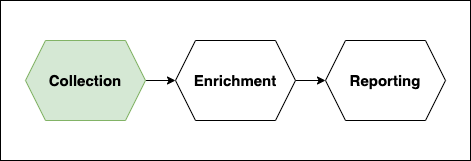
\includegraphics[width=\textwidth]
{figures/data_flow.png}}
\caption{\label{fig:my-label} Data Flow}
\end{figure}



As of today there are, roughly speaking, three ways to collect data - professional measurement, remote sensing, and crowdsourcing. It is to the last of these three that we will direct our attention. 

Consider for a moment that the global population has exceeded 7 billion. This is an enormous number that is very difficult for our hunter gatherer brains to grasp so let’s think about this in a slightly different way. Imagine that you’re in a large city square with ~1,000 people (besides yourself) milling about and you’re looking for someone with an interest in the biology of mushrooms. Now suppose only a single person in that whole crowd fits the bill. Pretty disappointing right? Not really. Even if only 1 out of every 10,000 people on the planet had an interest in the biology of mushrooms that would make for a force of over 700 thousand people. To put this in perspective the entire population of the city of ancient Rome was somewhere around 500 thousand. This is the power of crowdsourcing. With today’s population, even if only minuscule fractions of people take interest they can still end up representing workforces that whole societies would’ve had trouble pulling together in the past. 


\begin{figure}[!htb]
\center{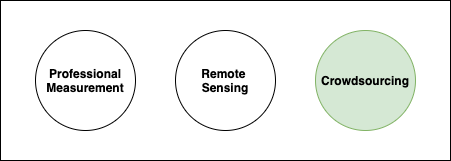
\includegraphics[width=\textwidth]
{figures/categories_of_measurement.png}}
\caption{\label{fig:my-label} Categories of Measurement}
\end{figure}


This crowdsourcing power is already being wielded for earth stewardship through applications like eBird, iNaturalist, and Nature’s Notebook. Apps like these give people across the globe an opportunity to help collect data about their local environment that has been used to create real, scientific knowledge and management programs. Yet, while these apps are phenomenal they have only begun to scratch the surface of the full scope of data we could obtain from crowdsourcing (in this case known better as citizen science) to help drive our understanding of our biosphere. So, in order to drive this forward the question we must ask ourselves is simply this - what barriers are there to entry into this space? The answer is unfortunately rather daunting.

To see why this is, let us put ourselves in the shoes of someone wanting to start curating a new kind of crowdsourced data. First they must determine what kind of protocol they wish to give users to use to collect the data. This part of the problem is no issue as this is well within a steward’s wheelhouse. The problems arise when considering how to get this protocol to users in a scalable way. Distributing a protocol across a country or across the globe means an application will need to be built and as with all applications there will need to be a UI, a database, APIs, proper security, authentication, styling, … you get the idea. For someone not versed in application development this is daunting indeed. And, when you consider the fact that this application will likely need to be supported across several different platforms, the headaches and worries just multiply. But it doesn’t end here. Even if the app gets built there’s still the issue of drawing users to it. Now our poor steward has to consider adoption strategies and driving and maintaining engagement. Successful applications take teams of developers to create and support - and for a reason. 

So what can we do about this? Well, when you look across the crowdsourced data apps that already exist in this space, one quickly realizes that the only differences between them are the protocols used to collect the data and the portals used to subsequently view and engage with the data collected. Otherwise everything else, including much of the user base, is simply duplicated over and over again.

So suppose instead that there was a platform built that implemented all of these redundancies just once, hosted these varying protocols and portals, and took on the mission of driving discovery and engagement much like Spotify or youtube drives discovery and engagement of its content? Then suddenly our stewards don’t have to worry about building an app or building a user base from scratch but simply need to develop protocols and portals - the bit that, once again, is well within their wheelhouse. This would all but remove the barriers to entry into this space and provide the catalyst for crowdsourcing all sorts of data that could drive forward our understanding of the biosphere. Even for the user this is a better deal as they can create their own personalized citizen science hub instead of having to spread themselves across a whole variety of different applications. 


\begin{figure}[!htb]
\center{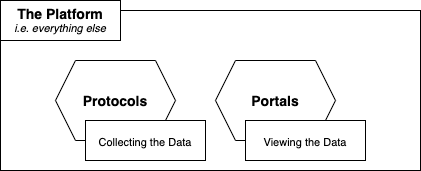
\includegraphics[width=\textwidth]
{figures/the_platform.png}}
\caption{\label{fig:my-label} The Platform}
\end{figure}


The mission then is clear. To catalyze our ability to crowdsource data from around the globe we need a platform whose mission entails two factors:

\begin{enumerate}
\item Consolidating everything that’s currently redundant
\item Driving discovery and engagement amongst the various protocols and portals
\end{enumerate}


\textit{December 15, 2021}

\section{Flokk Design Log - Joining the Ecosystem}
In the last Flokk post we arrived at the following summary:


Flokk would be a platform to host protocols and portals that would achieve the following two goals:
\begin{enumerate}
\item Remove the redundant parts of building an application
\item Drive adoption and engagement across the various protocols and portals
\end{enumerate}

Let's now look at each of these goals in the context of the tools that already exist.

\subsection{Removing Redundancy}
Building a citizen science application requires a few key ingredients: a UI (and all of its styling and design), a backend (with cache, database, API, etc), authentication, security, a data model, somewhere to host, etc. Now if you are familiar with the citizen science applications and software bootstrapping libraries that already exist you'll know that you can cobble together many of these components. For example both iNaturalist and SciStarter have authentication that you can piggy back off of. iNaturalist and GBIF both provide APIs that let you use their data model and backend. Flask-RESTful makes building APIs incredibly easy and Flask has several other plugins for building out other components quickly. If you insert data in well known platforms like iNaturalist and add the right meta data, that data will flow into other portals like Globi. The point is that while all the bits and pieces may be a bit scattered, most of the tools to put together a citizen science application already exist and just need to be cobbled together. Which brings us to the following conclusion:\linebreak

\textit{Catalyzing new application development is not about building new tools but about making it easy to discover and use the tools that already exist. }\linebreak

In other words our goal in Flokk should not waste its time replicating all of the great work that's already been done but make the tools discoverable and, especially for someone new to these kinds of things, accessible. 

\subsection{Driving Discovery and Engagement}
In a similar vein to the last section, the central driving observation here is that so many amazing applications (protocols and portals) exist. Flokk should take advantage of this ecosystem, not exist in ignorance of it. Indeed there are already so many great apps built around this ecosystem already. For example iNaturalist has a series of associated applications like Seek, Globi, or Caterpillar Counts that enrich their data, protocols, and experience. Yet, unless you know what to go looking for you'd never find these apps! This underscores the need for a place where all of these various applications and tools can be linked together and made discoverable. If you're working on a project concerning insects within iNaturalist you shouldn't have to stumble across Caterpillar Counts. If you're making multi species observations Globi should be recommended to you. What we need is a marketplace that helps you navigate the vast array of citizen science projects and apps, provides recommendations, and links together apps that synergize well.\linebreak

\textit{Driving discovery and engagement will come from building a marketplace for citizen science tools and applications that links together relevant apps, provides recommendations, and helps you navigate the vast space of projects. }\linebreak

Wonderfully SciStarter is working to do exactly this! The already have and are developing a recommendation engine and have a vast catalog of citizen science applications and projects that they are enriching with metadata meant for enabling navigation. Rather than having to solve this problem ourselves we can simply go support them!

\subsection{Marketplace Engagement}
One challenge that popped into my brain while I was looking at SciStarter was that of keeping people engaged in the marketplace itself. As a very personal example I actually used SciStarter several years ago to find some citizen science projects. Subsequently, because my attention was focused on the projects SciStarter helped me find and not on SciStarter itself, I actually forgot SciStarter existed. I only rediscovered it recently! Keeping people engaged with a marketplace that they use to find things outside of the marketplace that will draw their attention for a long time is a tough problem and one that'll need to be solved in order to allow the marketplace to really drive continuous and thorough adoption and engagement\linebreak

\textit{A central challenge for our marketplace is how to keep people engaged with the marketplace when the marketplace is effectively driving their attention elsewhere.}

\subsection{Pulling it All Together}
Okay, let's go ahead and summarize our findings:
\begin{enumerate}
\item We have a series of refined tenets
\begin{enumerate}
\item There are tons of components for quickly building out citizen science apps that already exist. They just happen to be scattered about, so Flokk needs to make them easily discoverable and accessible.
\item Discovery and engagement will come from building a marketplace that links relevant apps together, provides recommendations, and makes the space of citizen science projects more navigable.
\item Such a marketplace needs to find a way to keep folks engaged, especially given the purpose of the marketplace is effectively to direct attention elsewhere.
\end{enumerate}

\item There are already folks working on these kinds of problems that we can work with! (How exciting)
\begin{enumerate}
\item SciStarter is driving after that marketplace.
\item iNaturalist, GBIF, Flask, etc. have built and are building the components necessary to make building new apps quick and easy.
\end{enumerate}

\end{enumerate}


\subsection{What's Next}
With all that's been said it should be clear that Flokk, above everything else, is about making things discoverable. Whether you're a scientist looking for components to reuse in your citizen science app or you're a citizen looking for new projects and cools ways of viewing your data, Flokk should make finding things super easy. Given this is all about creating that marketplace, and in the spirit of jumping into the currents that already exist, getting involved in SciStarter development seems like an obvious next step. 

That being said, you can't guide people on a trail you've never taken, or teach people a skill you've never used. So actually building an app with the aforementioned components is an  obvious next step as well. Through the experience of building such an app we'll be able to identify what works well, stumbling blocks, missing components, and how to best guide folks through the process of using these components.  

Finally, it is highly unlikely that every component ever needed has already been built. It is also highly likely that the folks in the best position to build these components will be the organizations already hooked into the field like iNaturalist, GBIF, and the like. Therefore becoming involved within these communities is another obvious step forward. 

\textit{December 21, 2021}

\section{Freeing the Mind with Machine Intelligence}
Technology has accomplished many wonderful things, but one thing I'd like to focus on is the value of automation. Whenever we manage to automate something we can deploy it at scale and move onto using our human brains to work on more creative and thoughtful things.

A relevant example of this is the monitoring of wildlife with camera traps. At first scientists had to spend quite a lot of time going through photos, many of which had nothing of interest in them, looking for and then identifying wildlife. This obviously limited the scale of the camera trap surveys and took valuable time away from actually interpreting and reporting on the data. Nowadays, computer vision is used to comb through the many tens of thousands of images produced in any particular camera trap survey. This both frees up the scientists to focus on using their creative, thinking capacities while allowing for far grander scale and continuity within the survey itself. Indeed, entirely new applications of camera traps become possible with machines in the loop. For example camera traps can be used as continuous monitoring and alerting systems if there's a machine brain watching at all times. 

This example rather nicely illustrates a standard part of any scientific process - transforming data from raw into more meaningful forms. Data is almost always captured in the "raw" because doing so is cost effective. Taking pictures is easy; having someone sit out in the field and count wildlife over days or weeks is not. But while raw data is cost effective it usually lacks the context and meaning required to weave narrative with. So the data has to be "enriched" into more valuable forms. 

When you think about it, though, this enrichment is really just a transformation of some kind. A big vector of data X goes in and a vector of more meaningful information Y comes out. And the function F which does the transforming is the menial task that, if automated, would allow our stewards to spend more time exercising their humanity while making deploying F at scale possible. So therein is our question - how do we go about creating machine based transformations really easy?

\subsection{Enter Machine Learning}
The first thing we must ask of any of these transformations is whether there are a clear set of rules that can be followed. If that's the case, then all we need is some code and we're done. But if the rules are not clear or at least not clearly coded we need a different tool - machine learning. 

Machine learning is by definition all about allowing a machine to learn, for itself, the relationship between a set of features X and a set of targets Y. Which is exactly what we're looking for! Now typically machine learning is looked at as something quite difficult so given  we want to make creating transformations easy we've got to ask ourselves what makes machine learning difficult? 

Given all of the research that's already been done on machine learning, today (in my opinion) machine learning remains difficult largely because of the vast array of options out there for how to tackle a problem. You must:
\begin{enumerate}
\item Choose a good representation of the transformation you want
\item Have enough data to teach the machine with
\item Choose good features
\item Choose good normalization and data cleaning patterns
\item Choose a good model
\item Choose the right parameters for that model
\item Choose the right evaluation strategy for your model
\end{enumerate}

Let's take a look at each of these in turn and see what we can do to make life easier for ourselves and our stewards.

\subsection{Tackling Difficulties}
\subsubsection{Getting Data}
Machines need training data to work with - that is cases which have been labelled with ground truth. A good example of training data would be photos already labelled with what's in them. Getting training data is perhaps the most difficult part of any machine learning problem and this is especially true in our particular case. Remember the whole reason we're here is that simple rules didn't cut it - which means we need humans in the loop and humans are typically expensive - particularly if they have to be professionals. Thankfully, like with data collection, citizen science can come to our aid as a way to get cheap (if not free) crowd-sourced labels for our data. Websites like zooniverse already allow for folks to post data that needs labeling in a community of citizen labelers! 

Unfortunately there's a catch. Crowdsourcing works when the task is simple enough for someone with little to no training to accurately do (like identifying if something is in an image or not and where it is) but sometimes a particular label can only be provided by an expert. For example, suppose we've got pictures of two subspecies of elephant. You might not expect the average person to know which is which consistently. In these situations we need to do everything we can to use the expert's time as efficiently as possible (not that we'd use crowdsourced time inefficiently, of course).

Thankfully there's an answer to this call in the form of Active Learning. This is a paradigm of human in the loop machine learning where the machine determines which data points (for which it doesn't have labels already) would be most useful for its learning. These model chosen examples can then be sent to humans to be labelled, the model can retrain itself with the new information, and the whole process can repeat. In theory this means that you don't have to label as much data because the machine is being specific about what it actually needs to learn.

So, with citizen science and active learning we can significantly reduce the headache to our stewards in creating the data we need to train our models. 

\subsubsection{Choosing the Right Parameters}
All models come with a series of knobs called hyper-parameters. By turning these knobs we change the specifics of the model and therefore its shape and flexibility. Thankfully there are many standardized procedures in place for automatically tuning these hyper-parameters. So we can make these procedures standard and allow our stewards to get on with better things.

\subsubsection{Choosing the Right Model}
Today, for the vast majority of problems, there are already a pretty standard set of well developed models and model architectures. Put another way, if you know the problem you are dealing with, a handful of models are all you really need to know about to get most of the bang for your buck. Better yet all of these models follow more or less the same APIs so you can build, train, and test all of them with the same code. What this means for us is that your steward only needs to specify the kind of problem (computer vision, classification, regression, time series prediction) and we can choose the best model by simply building the full handful and selecting the best out of the bunch. Yet another thing automated away!

\subsubsection{Choosing Good Features}
Features are the specific representations of the data that you want the machine to use. As such they themselves are actually transformations. So if you have your raw data X, features (and indeed normalizations) really create a new vector U  that is given to the machine to produce Y. Given that we've associated our labels with X and not with U, features can really just be swapped out ad hoc without disrupting the rest of our pipeline. This means the only "difficulty" that comes with features is just creating them in the first place but this is always a creative endeavor and thus totally belongs in the human realm. In other words everything but the creative part has already been automated away by associated our Y directly with X and by making model selection, training, tuning, and testing automatic. 

\subsubsection{Representation and Evaluation}
Evaluation for its part is easy. Our stewards just need to select the criterion for evaluation (something a machine should never do on its own) and then the rules for that evaluation are coded up. Over the years dozens of such evaluations have been dreamed and coded up and it's highly unlikely that stewards would need something new.

As far as representation is concerned this is a place where humans must be the ones making the determination. You can't expect anyone (and especially not a machine) to know what to do if you don't tell them. What's interesting about this part of the problem is that if it's difficult to actually figure out what you want the machine to do you probably have no idea what you're doing yourself. And if you don't know that, you can't automate it. So this bit should be easy once you know what you're automating. 

\subsection{Summary}
Okay that was a lot. Let's summarize. 
\begin{enumerate}
\item Representing the problem is only hard if you can't describe what you want automated.
\item There's already a vast array of evaluation techniques - why not just allow our stewards to pick one?
\item Gathering labels for data is expensive. We can make it less so by engaging citizen scientists to crowdsource labels and using active learning to allow the machine to direct the humans to the training it needs the most. 
\item Even if we had a model selected, we'd still need to tune its hyper-parameters. Thankfully well established, automatic procedures already exist for this.
\item Thanks to all the research that's been done, for any particular kind of problem there's a handful of agreed upon best model candidates. Thanks to the fact that they usually share APIs we can simply train them all and pick the best one. Model selection automated.
\item By associating our Y directly with our X and by automating selection, tuning, training, and testing of our models, the only manual part of creating features and normalizations is actually building them - which is an entirely creative process and thus one better suited to humans anyways. 
\end{enumerate}

Effectively then, all this represents is pulling together existent tools and knowledge into a framework that allows for plug and play features, built in model selection, tuning, training, and testing, built in active learning, and easy accessibility to crowdsourcing. 

With this framework in place we'd have automated everything about building transformations except the bits where we absolutely need humans in the loop. Then with these automated transformations in hand we can deploy at scale and let our stewards get back to the creative, thoughtful work we, as humans, excel at. 

This is project Kameleon. 


\begin{figure}[!htb]
\center{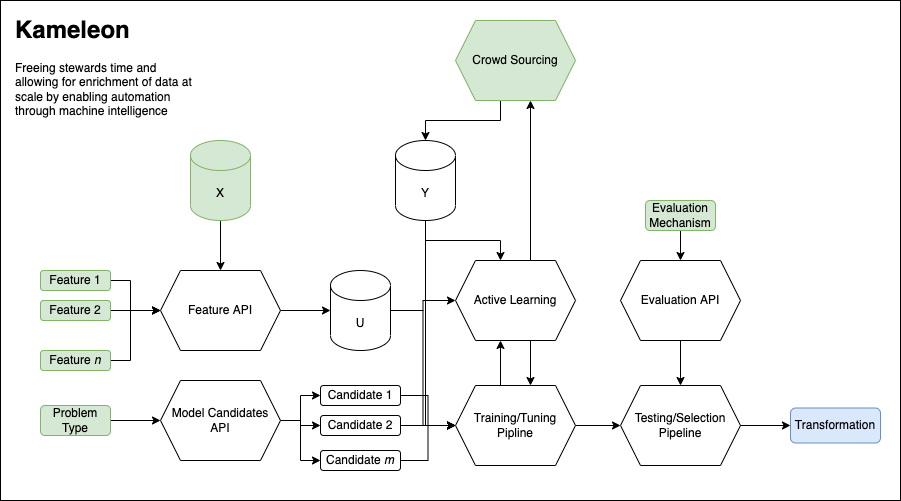
\includegraphics[width=\textwidth]
{figures/Kameleon.png}}
\caption{\label{fig:my-label} Kameleon}
\end{figure}


\textit{December 26, 2021}

\section{Creating Allies and Building World Views}
So far we've discussed what it takes to put together management plans, but we haven't spoken much, if at all, about taking action to see those plans through. Obviously given the crisis we find ourselves in, effective action could easily be considered the most important part of this problem. 

Recently (December 2021) I did a google search to find books on taking action and found lots of books speaking to the in-action that exists today around this crisis and plans to get around it. How to Save Our Plant, As the World Burns, and How to Avoid a Climate Disaster being just a few of the titles. Obviously then if you want to know what should be done it isn't my rambling thoughts you should be reading. 

But, as I have a habit of doing, all of this reading got me thinking about underlying causes for the situation we find ourselves in and how we get ourselves out of a rather self destructive loop. Many of the books out there demanding climate action focus (rightfully so) on what needs to be done immediately to prevent us crossing a point of no return. But my question is - why are we here in the first place? And more importantly, what can we do to make sure we don't end up here again? Here, my mind quickly turned to evolution.

Cultural evolution that is. In my mind (and this is 100% an opinion) the state of our society at any point in time is the result of the cultural pressures that define the "survival of the fittest". In other words if you want to understand why a culture is the way it is - i.e. what kinds of values, organizations, infrastructure, etc. it has - you have to look to what causes one thing to be able to outcompete another. Competition is at the root of everything, whether we notice it or not. Just the fact that two kinds of organization or idea exist in the same niche means that there are backers for each that are effectively competing for their space to exist. What ends up winning is determined by the nature of the forces of competition. 

So what drives this competition? Where is the source of its energy? Well for culture it comes back to people. For us in a capitalist republic the people of import are the ones who vote with either the dollar or the ballot. They are the ones who power the ultimate fate of corporations, governments, and values. If people stop paying for the goods or services rendered by a corporation, that corporation will cease to exist. If voters choose to not re-elect an official, that official loses their seat. To be clear, this is not to say each individual has the same power as the next, votes mean different things depending on where you live and who you are, and money is obviously very far from evenly distributed, but the principle still stands - the voter, by dollar or by ballot, underpins the forces of competition and therefore the direction of culture. 

Yet having the power is not the same thing as wielding it. People buy things and vote on the basis of their worldview (values and sense of how the world works). Yet that worldview is constantly changing as people have new experiences, absorb new information, and just generally keep on living. And given that a single dollar or ballot isn't going to change anything on its own, it is the trends in world views (cast into the unbiased distribution of voting power) that really defines the competitive forces in our culture. In other words, it is those who influence and build world views that are actually wielding the forces that shape cultural evolution. 

Given this admittedly very philosophical calculus we arrive at the following conclusion. The reason our society exists at it does today, the reason we are in this self destructive loop, is because the entities winning at building world views that turn into voting action (with dollar and with ballot) are not ones with long term interest in the health of our society. If we want action to be taken effectively we need to be winning at building world views within our cultures. 

So how to do this? Well I once read a very interesting book on the lifecycles of trends (the name of which I'm unfortunately forgetting now, but if I ever remember it I'll be sure to come back and cite it here). One of the major lessons I took away from it is that the majority of people don't take on views or behaviors that are viewed as new or strange - instead they need to see others taking those same things on successfully first. In other words action happens along a gradient - you start with people who are predisposed to toward that action and then work your way along the gradient until you eventually get to the intractable. Framed like this taking effective action is therefore about finding allies at your particular point in the gradient and then facilitating them in moving everything along to the next step in the gradient. 

So imagine this. Imagine a platform where stewards with new management plans, and therefore some new worldview to build, start by going and getting matched with people who are predisposed to take that kind of action. In other words, they're able to easily find their trendsetters. Then imagine that that same platform facilitates a kind of teacher - apprentice relationship where these new allies are trained up and facilitated by the stewards to become mentors and activists themselves. Then once the first group of people are trained up, they can get matched to people relevant to them, one step up the gradient, who they can now mentor. Rinse, wash, and repeat. In this manner we'd be able to facilitate the creation of new components in the cultural worldview while also avoiding the problem of overwhelming our activists because the matching could be specific enough to target the kinds of problems our allies would really enjoy and be effective at rather than throwing every problem out there at them. And as a plus this platform wouldn't need to be biased toward a particular point of view. Instead it could just be a means for training up well educated, well supported advocates of various ideas which could then compete more equitably. Or at least that's the thought. 

Well it turns out I already had this idea but, to summarize:
\begin{itemize}
\item The nature of world is defined by the forces of cultural evolution
\item And in a capitalist republic those forces come in the form of votes - by dollar or by ballot
\item Those votes are wielded according to the worldview of the voter, which means that the worldview builders are the ones wielding the forces of cultural change
\item We're in the state we're in because those who care about our long term future are not the current winners of worldview building
\item But changing worldviews is all about finding allies in the gradient from accepting to intractable, and then facilitating those allies in moving the ideas and actions along the gradient
\item So what if we made a matching/facilitation platform that could match mentors to mentees, facilitate their development, turn prior mentees into new mentors, and then allow for a snowball effect?
\end{itemize}

This is project Mycelium.


\textit{January 9, 2022}


\section{Citizen Stewardship - consolidating the roadmap}

Thus far we've described three general projects under the umbrella of Fjorgyn - Flokk, Kameleon, and Mycelium. Each of these, in one way or another, tries to take advantage of the scale and power provided by the citizenry. If you think about it though, the folks involved in any one of these projects are likely the same. If I'm interested in helping develop the science around a coastal system near me, I'm probably also interested in activism around that same system. Indeed if Flokk is aware that I should be recommended a protocol or set of portals, it's not a far leap to say that I should be recommended the related activism too. The audience in Flokk, Kameleon, and Mycelium are all the same which leads to a rather useful summarization of Fjorgyn thus far:

Project Fjorgyn is fundamentally attempting to do just two things:

\begin{enumerate}
\item Create an active and engaged audience around biosphere stewardship
\item Facilitate the integration of this audience into biosphere stewardship
\end{enumerate}

In other words, Fjorgyn is an ecosystem for the proliferation of citizen stewards.

The distinction then between Flokk, Kameleon, and Mycelium is not in what they are fundamentally trying to do or who they are trying to reach, but rather which step in biosphere stewardship they are trying to catalyze through citizen involvement. At the end of the day, they are different aspects and features of the same ecosystem. 

This is a very useful thing to know because the features in each of these are only useful with the audience that surrounds them. In other words for Flokk to be valuable there have to be a lot of citizen scientists. For Mycelium to be useful there have to be a lot of activists. All of these projects are dependent upon large user bases. But what this summarization tells us, is that if we are successful at building an audience in any one of these areas we are effectively being successful at building out the audiences needed for the other areas as well. By solving this problem in one situation we more or less solve it in all three. 

Thus, in the same way that our summary of goals divides into two points, the development of Fjorgyn divides into two as well.
\begin{enumerate}
\item Building out a community of engaged citizen stewards (using any or all of the areas identified)
\item Building out the features that integrate these stewards with the various areas of stewardship
\end{enumerate}

This then consolidates the roadmap of Fjorgyn into one stream. Rather than building out three ecosystems we are actually building out one with three different feature sets. By building out any one of the feature sets we can build out the ecosystem and then, as we gain traction and development resources, we can expand into the other feature sets. All the while, the ecosystem is consistently getting built and the community growing. 

Fjorgyn then is not about building citizen scientists, or citizen developers, or citizen activists in particular - instead it is about building full fledged citizen stewards.


\textit{January 24, 2022}

\section{Biophile}
I recently decided it would be good practice to replicate some studies around ecosystem services - just to get experience with how people have done these kinds of simulations and predictions myself. So I pulled up some studies relevant to my area and began enumerating the services so I could choose a particular project of most interest to me. Air quality, water quality, climate control, food, the list became quite extensive. But, as I was sitting there, I began to realize something - nothing on this list was why I was writing this list. I didn't stumble into this cause on account of water quality or desertification, I am here because I absolutely adore my local biosphere. And as I thought about it more, it occurred to me that everyone I know who has really cared about this stuff and fought for it was in the same boat. Sure, ecosystem services and the associated modeling informs and fuels our fire, but at the end of the day it is not the fire itself. No, the fire is always a deep set love that would exist separate of all of these "services". For some people it's fishing that they love. For others it's going out hunting for mushrooms. For me it was originally just catching frogs. That love for the critters and plants that make up the biosphere is where this passion really comes from. 

We know today, just given how people vote, that the biosphere is not a priority for most people. It just isn't. And so folks have tried a different tact - they try to identify what is a priority and then link that back to the issues our biosphere is and could end up experiencing. Worried about taxes - well your government is going to need more money from you as it becomes harder to live on this planet. Love sushi? Our management strategies may mean you don't eat tuna 10 years from now. We trying to convince people they should care by linking what we care about to what they care about. 

Yet, as we've seen, there are so many ways in which this can not go as planned. People may not fully appreciate the full impact and scope of the argument. They may not trust the source or feel like it's overblown. Given all of the different arguments being made they may simply become overwhelmed or shutout the information entirely. And then there's the fact that when they go to vote or buy something that information has to be on the forefront of their mind to really make a difference. And then beyond all of this, there's the fact that even for those people who are convinced - the basis of their fire is not any of these arguments, but rather the fact that the biosphere was just a priority for them to begin with. Which all points to the following conclusion - if people are to make the biosphere a priority, convincing them that it's secondarily valuable is not going to cut it - they have to love the biosphere for itself. 

Within this frame of view it becomes glaringly apparent why our world is having so much trouble doing the right thing. What opportunities, what forces really exist to drive this kind of adoration? In high school, biology is about mitochondria and anatomy, and only briefly and dryly covers ecosystems or biodiversity or any of the other myriad components of our biosphere. In college, unless you study biology, the subject is just ignored. And then from there, there's just nothing. Field guides take dedication and prior want to parse and understand. The wonders of our natural world are almost always painted as being in some far distant corner of the world. And the news only speaks of doom and gloom. Where is the opportunity to build biophiles? 

If we want a world filled with people who actually prioritize the biosphere in more than words (and only such a world sees a shift in consumption and voting patterns) we have to take concerted efforts to build deep, personal love for the biosphere. Without that kind of emotional connection all of the tools we build, all of the science we do, will forever be thrown into a world full of people who, fundamentally, don't really care and will consistently end up prioritizing the things that do matter to them. But building up this kind of love is not about rational arguments or running through the science. It is about kindling that same kind of adoration and wonder I had as a child sneaking along the edge of a pond catching frogs. Reconnecting people to their local, natural world and helping them fall in love with it - that's the way out of our current dilemma. Because at the end of the day our societies are a reflection of our cultures, and until our cultures are steeped in connection and adoration for the biosphere our policies, businesses, technologies, and actions won't be.

We need to reconnect. 

\textit{January 28, 2022}

\section{Reconnection through Adventure}
Last time I wrote, I made the observation that in order for there to be a culture that values its environment, individuals must fall in love with the wonders of their world. I would like to expand upon this with a few short observations.

In mulling over the kinds of activities that fall into this category with any kind of generality that two conditions are necessary (if not on their own sufficient). First, these activities must be flow inducing. This is unsurprising as flow is effectively equivalent to fun itself. The second condition is that they be social. From sports, to seeing the movies, to going rock climbing at the gym, all things in which people generally take consistent joy are social in one way or another. This too should not be surprising as we are, after all, social creatures at our core. Indeed taken together, these two conditions provide a powerful formula which feeds both our desires for fun and for companionship. If we hope to connect people to the wonders of their environment we should take stock of these two ingredients of success. 

In mulling over the kinds of activities that fall into this category with any kind of generality, it becomes clear that two conditions are necessary (if not on their own sufficient). First, they must be flow inducing. This is unsurprising as flow is effectively equivalent to fun itself. The second condition is that they be social. From sports, to seeing the movies, to going rock climbing at the gym, all things in which people generally take consistent joy are social in one way or another. This too should not be surprising as we are, after all, social creatures at our core. Indeed taken together, these two conditions provide a powerful formula which feeds both our desires for fun and for companionship. If we hope to connect people to the wonders of their environment we should take stock of these two ingredients of success. 

The next observation is that in order for the connection built to have the desired effect (a populous interested in caring for their environment), it must be more than skin deep - it must be informed and rich in understanding. To put it more simply we must not only get people out into their world, but give them subtle familiarity with it. And this means instilling knowledge. Specifically, we are concerned with instilling knowledge that keeps. 

In my experience there are two ways to do this. The first is by practice - practiced knowledge is kept knowledge. But here, in our specific situation, we face a problem - practiced knowledge in the environment, at our scale, quickly becomes the destruction of that self same environment. If whole towns took up foraging, or hunting, or even life listing for that matter we'd quickly lose our flora, our fauna, and flatten the environs around us. Especially around population centers we far exceed the carrying capacity of the surrounding habitats. So instead of practiced knowledge we must look to something else - power narrative. The construction of wonder through narrative and performance is an extremely powerful tool for instilling knowledge. Indeed I count it as the reason why the average person knows more about fictional places they know about than their own world. No one has cast a spell and yet there are hordes of people who know exactly how too if they could. 

And within a world as wonderful as our own powerful, awe inspiring, biosphere, narrative is not hard to come by. Indeed our whole world is like a vast theatre with countless cast members and an ever changing series of plots, stories, and sub plots. It is just that today, there is no playbill, no theatre guide, and no calendar of performances readily accessible - especially for one's local environment. And herein we find a solution to fulfill all of our observations.

Suppose that someone created that playbill and orchestrated the events. Suppose there were regular adventures to partake in within your broader area. Adventures that would showcase the various stories and dramas being played out around us - stories forever changing across habitats, biomes, and seasons. Suppose those adventures, like many more athletically focused ones today, included time during or afterwards to break bread with your newly found companions and share stories, laughs, and company while having a drink or two. Such adventures could be scheduled with astonishing frequency and consistency given all there is to see in our grand backyards, and could be made to be exceedingly social. With carefully crafted narratives that let the natural world steal the show, understanding and wonder could be instilled, and if that didn't count for enough flow, the hiking, kayaking, snorkeling, and general outdoorsmanship required to partake in these kinds of things has already proven its worth as a flow inducing mechanism. And throughout all of this, and especially with the opportunities for interaction around food and drink, it could be made social and consistent so that people could come to depend on it as a place of fellowship as well. 

In this way we'd be able to provide a bridge into the wonderful world around us and work to create a consistent, repeating, relationship with the local environment that could be woven into people's normal routine. Presenting a varied host of motivations it could provide a bridge for people from all walks of life to learn all about the various other kinds of activities that exist within the environmental sphere from citizen science to environmental activism. This could be a place of common ground, a place of fellowship, and a place of joy where people can be reconnected with their world. 

\textit{February 28, 2022}

\section{Digitizing Guides}
As I go through the process of capturing identification logic for the trees of New England I can't help but be astounded by the amount of information and the effort it must've taken to gather it all up. I have discovered that there are over 101 native trees in my "backyard" split amongst around 26 families. I have also started to appreciate the innumerable number of things required to properly identify them and the combinatorial difficulties that come with capturing all of that. And, as I've read bibliographies and gone looking for this data online I've discovered the veritable armies of scientists who've been solicited to put all of this information together. And this is just for trees in New England! What of the mushrooms, insects, birds, wildflowers, mammals, and fishes in all of other corners of the world! Yet I know field guides exist for much of these too. I cannot even begin to guess how much effort has been put into collecting and organizing all of this information and yet, as far as I can tell, none of it is properly digitized!

Now by digitization I do not mean sticking a pdf somewhere (which seems to be what passes for "digitization" in most cases). I mean properly representing the data in a machine interpretable form that's easy to use, scalable, and doesn't require vast amounts of knowledge on the subject of identification. I mean shape files stored in easily accessible databases, not images of ranges. I mean clear timelines of phenology, and well documented and organized artwork. Imagine what could be done if this data was in such a form! 

Right now if someone comes up with an idea for a field guide, or phenology guide, or whatever other kind of guide, they must first collate all this information all over again! Or repeat all of research to get a slightly different version of it. If instead all of it was properly digitized you'd separate the gathering of the information from its presentation and use. People could devise all sorts of cool apps and applications for the data that could pull from well documented central databases. And their apps would simply grow with the information. Imagine how useful this could be in reconnecting people with their world. Imagine how many great projects could come of it - we'd only be limited by people's creativity!

Here then is another goal for reconnection - digitizing all of this interesting and wonderful information about our biosphere in such a way that the creation of applications can be disentangled from the collection of the data. If we could do this we'd vastly multiply the value of the herculean efforts already going into putting together these guides today. 

\textit{March 3, 2022}

\section{Bioverse 0.2}
I've had a brainwave and I wanted to record it here.

\subsection{The Idea}
Alright so the idea is for an app that has three components.
\begin{enumerate}
\item The first view in the app (and the place folks would start) is a phenophase view. Basically for the current time period (week or month) there'd be a list of "events" likely occurring near the user - things like flowering trees, migrating birds, fruiting fungi, etc. This data would get pulled from the National Phenology Network (NPN) or something similar.
\item Upon clicking on one of the phenophase + taxa pairs from the first view folks would be taken to a "where" view. This would simply be a map showing them where occurrences of those taxa have been found in the past. This data would come from iNaturalist or something similar. 
\item Finally there'd be a context and cues view that would give folks information on what to look for and where to look for it (think habitat cues) as well as additional information on the taxa. Wonderfully much of this information is in wikipedia!
\end{enumerate}

Okay so those are the views provided by the app. Why do I think this is so cool? Let's dig in.

\subsection{For the User}
\subsubsection{A Guide}
If you go to a new town for the first time and try to explore it without a guide you're basically leaving things up to chance. The restaurant you decide to go to may be an absolute dud, you may completely miss an amazing section of town, and you might not realize the right time of day to be in a particular area. This is why guides are so darn useful. The important thing is that they tie together time and place and give you the cues you need to find what you're looking for. 

The field is an absolutely wonderful "town" in this analogy, bustling with all sorts of wonders. But it's also sprawling and huge and what you get out of it is very, very dependent on when you happen to show up. Show up at the wrong time and you'll miss the migratory birds. Show up at the wrong time and you'll miss the magnolias flowering. So time is super important. Most guides to the field don't include this dimension at all. So by starting with the time dimension we immediately provide value by increasing the odds that when you do go into the field you'll get to see something awesome - we're actually providing a real guide to what can be seen.

The other two views give us the other necessary components for a good guide. First the guide needs to tell you where to go but given nature doesn't have an address we instead need to be able to inform people of the general areas they can go looking for things. The map view gives us this and allows folks the flexibility to pick a spot that suites them. 

Once they're there, they'll need the context cues required to actually zone in on what they came to see - thus the third view. But what's absolutely wonderful is that we can provide that context more or less free form because people are already focused in on a specific taxa. In other words we can go into far more depth that a typical field guide can because we know this is what the person wants to focus on. 

So all in all we've got a pretty great guide for getting out and about in the field and seeing cool stuff.

\subsubsection{A Dynamic Playbill}
The next awesome set of features is the dynamism of this guide. Because it's time specific, as the weeks and months pass the "playbill" will change and so there'll always be something new an interesting to go see. Anything static quickly floats out of people's brains, but something that's always changing has a better chance of keeping their attention. 

Then there's the fact that given we're tying into things like wikipedia, iNaturalist, and the NPN this stuff is just nation wide right out the gate! If you go to a different state for work or pleasure you can still pull this thing up and find some cool things to go and see!

\subsubsection{Clear Objectives}
If you were to sit down day one in your calculus class and the teacher just tried to shove every concept in your brain all at once you'd end up feeling overwhelmed, stupid, lost, and probably more than a little bit angry. Yet this is exactly what most field guides and field guide apps are like today! You take them with you outside and then just get hit by the 100s of species and 1000s of specimens you don't yet know how to identify or even organize in your brain! 

By focusing on specific phenophase+taxa pairs people will have clear objectives for what they want to see, what they're looking for, and what clues and cues to follow. And by having this lineup change throughout the year they'll be moving through different taxa one step at a time. As a result they'll still end up building knowledge of the various entities within the world around them, but instead of getting hit by it all at once, they can add things in layer by layer. 

Finally many species are hard to identify at the wrong time of year and this can lead to considerable frustration on the part of the amateur. By having people go out at interesting times during a taxa's phenology, identification will be far easier and the cues and clues needed far less overwhelming. 

All in all this'll make things far more bite sized and approachable. 

\subsection{For the Developer}
\subsubsection{Incremental Value}
Field guides are typically very onerous to put together because they more or less require completeness. If you want a field guide of trees you need to know about most if not all of the trees for that guide to be useful. In our case however this is turned on its head. Because we're focused on phenophase+taxa pairs when someone adds but a single pairing, we have something new and immediately valuable for people to go check out. This is an amazing feature because it opens us up for crowdsourcing. If someone is interested in just one taxa group and wants to add stuff for just that (and only the ones in their area) that's great! We can immediately use whatever they produce because we're not chasing completeness. 

\subsubsection{Just the Links}
In a similar vein, because we're taking advantage of applications that already exist (NPN, iNaturalist, and Wikipedia) there's no need for us to host any data or curate anything at all. All we've gotta do is present things nicely and link them together. On the one hand this makes the life of the app developer much easier but it also means that the means to contribute to the content have already been worked out. 

\subsubsection{Instantly National}
I already mentioned this but wanted to mention it here as well as it's just as valuable to the development. By using such tools as NPN, Wikipedia, and iNaturalist we get national data right out the gate. There's no need to build out separate apps for different regions, or curate data for different places, it's all already there!

\subsection{For the Environment}
This I think is the coolest part. If people actually engage with this application and use it regularly we'll end up building a cohort of people who are familiar with what's in their backyard not just as species but as individuals with life histories of their own. By getting to follow the various taxa through their life stages throughout the year, folks will be able to see them for the living, breathing neighbors that they are. In addition, by being able to direct people's attention to a few taxa at a time, we'll be able to give them a far great depth of context and thus increase the level of wonder associated with each species. This is exactly the kind outreach I believe we need in order to create a caring, understanding public. 

And as a plus they'll be introduced to the citizen science community and can see first hand how vibrant that community is as well as the gaps that still need filling (which they can help fill if they feel so inclined). 

\subsection{Conclusion}
All in all I'm really hyped about this idea. It's super easy to build, immediately national, perfectly setup for crowdsourcing, makes use of every new increment of information, connects people to the citizen science world, and, most importantly, gives people the guide they need to explore the wonder that is their local biosphere.


\textit{March 9, 2022}

\section{Precedent}
A sophisticated solution, while on the surface a problem to a specific and usually singular problem, is, below the surface, actually a solution to a grand number of things. For example suppose that you are building an app. As you are doing so, there are many things to consider:

\begin{enumerate}
\item How will the app scale?
\item How will the code get organized?
\begin{enumerate}
\item How can one organize the code for ease of use and discovery?
\item How will one document the code?
\item How will one make different components reusable?
\end{enumerate}

\item How will we deal with security?
\item How will we deal with theming?
\item How will we onboard new folks?
\item How... you get the idea
\end{enumerate}

In short, when we build great things, we are in fact satisfying an amalgam of different requirements and wants. And this means that when we bring new people onto the project we must ease them in by giving them precedent to copy, paste, and modify. Why? I'll give you three separate reasons.

\subsection{Avoiding Reinventing the Wheel}
Being able to know how to satisfy all of these constraints all at once is no easy feat. You, or whoever you learned from, would've gone through a great deal of trial and error to find the way in which to balance all of these things out, all at once. So even if you could somehow hand someone this full context all at once, actually having them develop a solution that deals with all of these would be asking them to go through the process of re-solving all of this. If instead you give them something to copy, paste, and update, they can solve just the new part of the problem instead of having to re-break all the ground you've already broken. And just imagine how slow things can get when every new person who comes along has to go through the months of trial and error each other person went through, just to get going. Providing precedent allows folks to build on what has already been figured out.

\subsection{Avoiding Overexposure}
In the above we assumed the person in question could just absorb all of the intuition, constraints, and goals all at once. But this is a ridiculous assumption for several reasons. First and foremost it would just be overwhelming - no one, and I mean no one, is just going to be able to absorb all of that in one go. So not only would they be overwhelmed when you try to shove it all into their poor brain, but when they invariable miss things and don't incorporate all that is needed into what they are building, you are likely going to have to tell them to throw much of their work away and try again - which is incredibly demoralizing. But, even if they could, in theory, absorb everything all at once there is another problem - communication, especially this kind of communication, is always lossy. No matter how hard you try there will always be things that end up miscommunicated, misunderstood, or just missed. And the only way to find those things is to act on the passed understanding and see where differences pop up. 

So imagine instead if we could give them all this context one bit at a time, iron out the misunderstandings, and then go onto the next layer of the context cake. This would make things far less overwhelming, lead to small changes rather than demoralizing restarts, and allow people to understand things bit by bit until they understand the whole picture. This is also accomplished by providing precedent. By allowing them to copy, paste and modify they can focus on one part of the context while the thing they are copying takes care of the rest. Then over time they can come to piece together the whole puzzle. 

\subsection{More Immediate Productivity}
Obviously another way of solving the above problems would be to give folks toy problems to solve. But toy problems rarely lead to real productivity - they are learning tools only. By giving someone something that's more or less complete they can still learn in a comfortable environment while also contributing back to the main project. This is obviously better for everyone involved. The person learning gets to know they contributed and folks can be helpful right from the start. 

\subsection{Conclusion}
Precedent - giving people something they can copy, paste, and transform - ensures that people can get running right off the bat, learn without getting overwhelmed, and prevents useless attempts at reinvention. Failing to provide it just sets folks up for long periods of time having to rework things over and over again, all while feeling they don't understand what's going on and that they aren't contributing meaningfully. So it goes without saying that when developing new members of a team you must pave the path with precedent. Anytime you cannot point to something they can copy, paste, and update means you should stop, pause, and look for precedent.

\textit{March 22, 2022}

\section{The Importance of Official Ownership}
Recently I've been thinking a lot about the role of responsibility within systems of organization. We've already spoken at reasonable length about the importance of clear modules and interfaces within the technical design of a system. But my question has been this - shouldn't the same apply to human systems?  

Imagine first that we have some kind of organization with enough complexity and work that no single person is going to be able to handle all of it. Indeed there's so much going on that many employees/individuals are needed to keep things running smoothly. Because of this multiplicity, people are going to have filter the organization around them. Which tasks do they take, which do they leave on the table? What information do they pay attention to, what do they ignore? 

If there are no rules for this filtering, chaos will quickly ensue. People will end up picking up the same tasks and stepping on each other's toes. Important information will end up ignored  for there is no completeness guarantee when people are filtering in an ad hoc fashion. And beyond all of this, the ignored parts of the organization may end up being critical to the value of the bits that are actually worked. Obviously there needs to be clear rules for this filtering that ensures coverage and completeness.

One of way of doing this would be to have a system which more or less randomly assigns work to individuals. Because that system could be aware of what all the work is, completeness and coverage could be guaranteed, but now a new problem arises. Within any kind of organization part of the "work" is figuring out what the new work will be. Doing that well requires vision and vision requires synthesis of information around a particular topic or component. So if folks are just getting hit with random tasks there's no opportunity for them to create this synthesis of vision. Therefore you'll end up with a queue of meaningless work and won't truly be taking full advantage of the creative element of your organization's individual brains. The obvious way to fix this of course is to ensure that the tasking and information flowing to any employee is more tightly coupled to particular subcomponents of your system. 

Alright so at this point people are working on particular subsystems, and enough people are in the organization to cover those subsystems. There's still one piece missing from all of this though. While our current setup could lead to vision it doesn't have to lead there. Just because people work on something day in and day out doesn't mean they'll take ownership for it. This could happen for lots of reasons - insecurities, lack of clarity around how ownership is attained, just simply being unaware of the need for ownership, etc. So the last piece to our puzzle is to make that ownership clear. In order for people to consistently step up and ensure the growth of a particular subsystem (or in order to note that someone is just not up to task) ownership has to be made official.

Okay, let's review. In order to not have chaos we've created clear divisions within the work and put particular people in particular spots. In order to allow for the shaping of vision (and therefore growth) we've designed these spots to be points of synthesized information and purpose. These two things together indicate that we've identified clear, divisible subcomponents of our system that have similarly clear interface points. Finally we've made it clear and official who is responsible for what within that system in order to empower people and also hold them accountable. In other words we've arrived at a point where the technical organization of our system and the human one are in parallel with one critical difference - whereas the technical system is defined using capabilities the human system is defined using responsibilities. This is because, on the human side, we want to clearly indicate the intention for growth. Besides this one difference, the technical vision and the organizational structure are parallel. 

Now before closing this out let's talk about one last thing - hierarchy. As we've discussed in notes of technical design, beyond the subcomponents there also needs to be coordinating components - a series of lego blocks lying around doesn't constitute a build. In a similar fashion our organization needs to have the responsibility of coordinating the individual owners assigned to a specific owner itself. Then, as the system grows (thanks to the vision and leadership of our owners) those subcomponents themselves are going to outgrow the capabilities of their original owners which will mean that the leaves in our tree of ownership are going to become branches and the original owner is going to take on the mantle of coordination amongst the subcomponents they've raised into being. In other words, hierarchy is the natural way to deal with organizational complexity. "Flat" organizations simply lead to uncoordinated subcomponents and thus eventual chaos and waste. In order to guarantee coverage and completeness a clear and official hierarchy has to be in place.

As a final note, we've spoken thus far as if the need for completeness and coverage is a given. But when you have lots of people working on different things, the only way to guarantee this is through clear accountability. Unless the bill falls to someone there's no guarantee that the bill gets paid at all. Each associated person can simply blame the group for letting something fall through the cracks. As a result singular accountability is incredibly important and yet another reason why official responsibility is a necessary component of organizational health.

In conclusion then, official responsibility and hierarchy that parallels the technical design of a system is a requirement to ensure completeness, coverage, coordination, and vision across the organization. It's also a requirement if you want folks in the organization to be both empowered and held accountable. So, the first step in creating a clear, healthy organization is the official assignment of responsibility and designation of a corresponding hierarchy.

\textit{April 16, 2022}

\section{An Empire of Biosphere Stewardship}

At this point, I think it's safe to say that biosphere stewardship is an existential problem for humankind. There's enough research (and frankly first person experience) to support this that I'm not going to try and make an argument for that here. Suffice it to say that if we don't take this problem seriously we will be inviting a maelstrom. 

A seemingly obvious conclusion of this, held by many environmentalists, is that the general public should be rising up right now and working to solve this grave problem. Indeed not doing so feels like a moral wrong. While I do not disagree that something needs to be done, I wonder if the placement of responsibility is misguided. 

Consider for a moment the fact that there are a whole slew of existential problems facing us today. World peace, hunger, poverty, education, human rights - just to name a few - are all equally large, equally intense problems facing our species today. Not only is there more existential breadth beyond just biosphere stewardship, but the depth of each of these problems is mind boggling as well. Biosphere stewardship itself is composed of climate change, mass extinctions, ocean acidification, pollution, deforestation, and so on. Furthermore, each of these problems exist on a wide variety of scales, from your neighborhood river to entire reefs, continents, and the whole atmosphere. How then, I ask, is any individual supposed to cover all of these things? How can we place responsibility for all of these on everyone? As I think is clear today, doing so is entirely non constructive and can only lead to anxiety and dismissal from the public as it's simply too much for anyone to actually fit in their brain.

	Placing responsibility for all the world's problems on the masses - and by extension the individuals composing those masses - is misguided and not constructive.

Okay, but these problems still need to be solved. So who should the responsibility go to? For me the answer is simple, the responsibility should be given to the vast segment of our population who already cares. In the past couple of years I've worked with tons of people who are volunteering their time and money to try and be a part of the solution. And what an array of people they have been - from all walks of life, ages, demographics, and skill sets. In sum, there is a ready population ready and eager to solve these kinds of problems.

What's the issue then? If there's this workforce already engaged in the problem why aren't we seeing the kind of movement we want? In my mind there's a simple answer to this as well - the efforts being contributed are sorely uncoordinated and unoptimized. 

If you read any meta studies on the conservation of species you'll quickly learn that the vast majority of our resources have been dedicated to birds and mammals with insects, crustaceans, and reptiles being all but ignored. If you go and look at your state government's organizations on ecological issues I'm sure you'll find (like I did in Massachusetts) a wide array of conflicting roles and responsibilities with lots of gaps in between. Many events (like cleanups) held by volunteer organizations work on relieving symptoms rather than solving the underlying problems. Scientific research often falls on unhearing or missing ears within governments. And mind you, there is no one actually working to coordinate the activity that is happening. In sum, lots of effort being expended with no guarantees of coordination or completeness. 

	There already exists a vast group of people who want to be a part of the solution, but there's no coordinated structure of responsibility for them to be a part of that guarantees completeness, a lack of redundancy, and that their work will indeed be part of a bigger picture. 

Now obviously creating this vast organizational structure for the whole problem is a behemoth of a problem. But perhaps we could start with a subproblem - like herpetology stewardship in the greater Boston area - and learn how to create such a structure within that subproblem. From there we could begin to expand and subsume other taxa and larger areas as we grow our way to create the full organizational picture. 

In summary, in order for us to tackle biosphere stewardship we must stop looking to "society" to rise up and take responsibility and instead create a clear and complete structure of responsibility for those already invested in the problem. By creating this "empire" of biosphere steward we'll be able to help ensure that the multitude of efforts and resources already being contributed to the problem are used in an effective, coordinated, and complete way. Through this we'll be able to ensure that biosphere stewardship is something that we can depend on happening, rather than leaving it up to fate as seems to be the case today. 


\begin{figure}[!htb]
\center{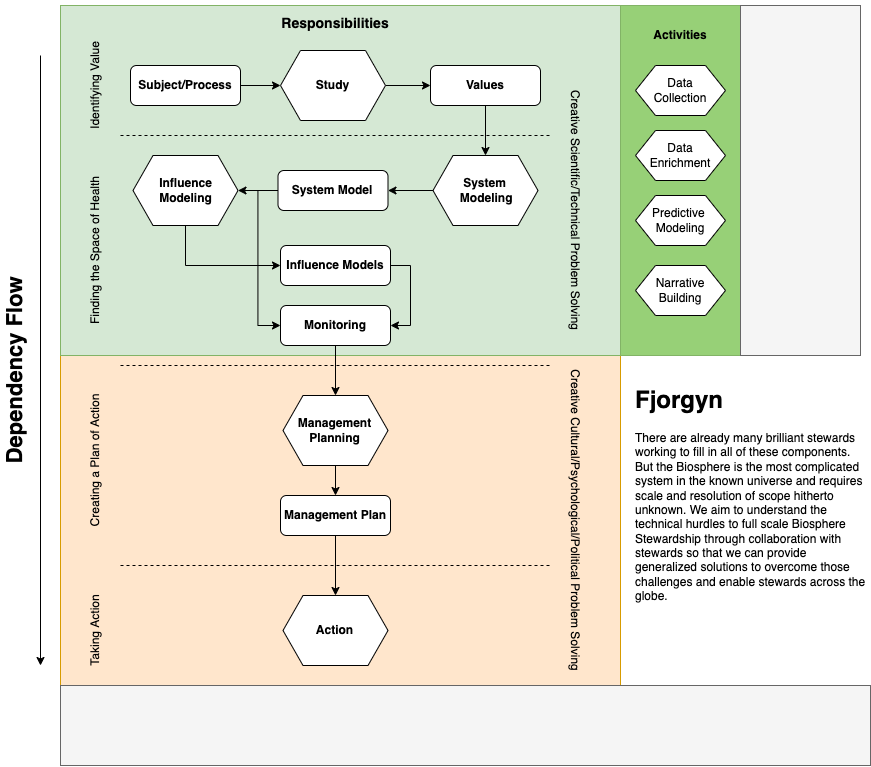
\includegraphics[width=\textwidth]
{figures/The_Flow_of_Biosphere_Stewardship.png}}
\caption{\label{fig:my-label} The Flow of Biosphere Stewardship}
\end{figure}

\textit{May 4, 2022}

\section{Organization of Research}
After having spent some time sampling articles within the realm of herpetology I've come up with the following organization scheme for research as it relates to stewardship. 

\begin{figure}[!htb]
\center{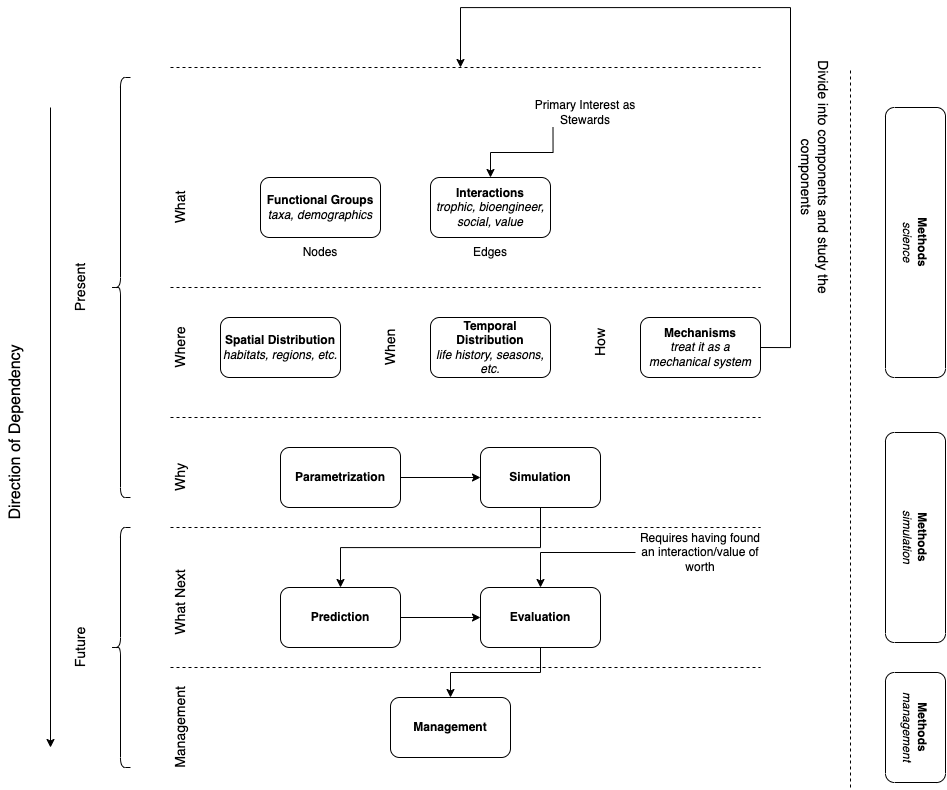
\includegraphics[width=\textwidth]
{figures/Categorization_of_Research.png}}
\caption{\label{fig:my-label} Categorization of Research}
\end{figure}

Note that, from a stewardship perspective, this all begins with appreciating some interaction moving from amphibians and reptiles (or some functional group subset) to the greater world that relates back to some fundamental value. Once this "value proposition" has been identified, we then flow through the rest of this chart to gather all of the information necessary to (as a first goal) be able to simulate and predict on that value proposition, and then eventually turn that into management plans. 

This then means that as a first step we can pick a particular interaction and the flow out from there, rather than trying to establish completeness at the top of this graph immediately. I believe this is the approach I will take to limit scope. 

\textit{May 5, 2022}

\chapter{Responses}
These are a collection of responses to readings.

\section{On Nonprofits and the Social Sectors}
\subsection{Lofty Missions, Down-to-Earth Plans}
In reading this essay, I realized two things: (1) I didn't have a clear, quick missions statement for my current intentions with Fjorgyn that I could rattle off in a heartbeat and (2) I wasn't in a position to quickly describe how I would measure Fjorgyn's success and filter opportunities as they came along. 

I really like the way the author described strategy as a filtering mechanism. This related back to the way I like to think about goals - not as something that you'll necessary ever meet, but as a way of focusing the time and energy in your life. As such, it seemed pretty reasonable to try to answer the two questions above. 

In terms of a mission statement I think I was able to cook something up that works well in relaying the goal, intuition, and vision behind what I would call the first phase of Project Fjorgyn:\linebreak

\textbf{We aim to improve the scale and cost effectiveness of biosphere stewardship by creating low-cost, easy to use tools and services for instrumentation and informatics.} \linebreak

This captures the fact that we want to improve scalability, and modernize stewardship with pointing fingers or blaming anything or anyone. It also describes the specific way we want to pursue this aim (out of the plethora of ways possible) and makes it clear we want to be the ones \textit{creating} those tools and services. Finally it helps focus us on the first part of the problem - gathering data and making it serviceable. Obviously once that data is there, there's much more to follow.

With the mission statement in hand the second problem is that of setting measurable goals and creating a real strategy around them - a filtering mechanism to keep Fjorgyn, as a nonprofit, lean, focused, and therefore effective. 

What I immediately found upon contemplation of this side of the problem is that it was most helpful to split things into two camps: (1) evaluation of the success of individual projects and (2) overall prioritization of the various possible projects possible. 

Starting with the former we can imagine a few stages in the lifecycle of one of these projects:

\begin{enumerate}
\item \textbf{Ideation}: at this stage we have a non-scalable part of stewardship in front of us and are trying to creatively think up all the ways more scale and cost effectiveness can be introduced. The outcomes from this exercise inform the work involved in helping out in this particular area.
\item \textbf{Removing Unknown Unknowns}: once some initial ideas have been settled upon, it's time to start building prototypes and judging their usefulness with real users of the tools or services. In this stage we really want to quickly find our way to a satisfactory MLP (minimum lovable product) while also mapping out the hurdles to creating such a tool or service.
\item \textbf{Deploying an MLP}: now it's time to just build the thing and start using it in the field. Getting this first generation out will then help us understand issues that arise at scale.
\item \textbf{Integration into Present Processes}: over time we keep updating the tools and services until they are just part of the norm for this kind of informatics problem. 
\item \textbf{Facilitating New Processes}: now that there's far more data we want to work with third parties who could take advantage of the data to make sure it's accessible and available in such a way that it empowers them. 
\end{enumerate}

Each of these clearly has it's own measurements of success and in some sense defines a turning point in the project where we must choose whether to continue or pivot to something else. That decision to pivot, however, requires a larger scheme for understanding the relative value and importance to the overall stewardship problem which of course brings us to the second part of our strategy - cross product prioritization. 

Here I think it's very important that we clarify the boundary of success for this first stage of Fjorgyn. While it is tempting to say success is the degree to which we are better stewards of our biosphere there are many components that make up such success. Therefore we must determine and focus upon the one having to do with instrumentation and informatics. 

\textit{In our case we are trying to create the knowledge required to make judgement calls.} Therefore this side of the project shouldn't be concerned with the relative importance of different kinds of stewardship, taxa, etc. It's job is really just to make the picture and perspective we have as complete as possible.

So in that vein we can see that the first task in creating a space of prioritization requires a cataloging of the space of knowledge and perspective that specifically details how complete each of those pieces are at present. We can start splitting by taxa and types of study and informatics to create a grid of sorts that describes the complete space. This in and of itself however is not enough to start prioritizing areas to pursue - equally important to the emptiness of a particular area is the difficulty in filling in the box. Want we to be able to pick are things that are low cost to address but significant blindspots overall. Furthermore there will certainly be synergies between different blocks as similar tools and services and can address whole groups of them. Therefore I propose the following stages to this process:

\begin{enumerate}
\item {Mapping the Space}: in this stage we are simply gridding out the full space of boxes in terms of taxa, informatics type, and region to understand where our blind spots are at the present day.
\item {Reuse in Present}: here we look at the tools and services already available and see if we need to simply facilitate their use or make small modifications to address particular blocks. The idea here is to understand whether small adaptions or reorgs can fill the wholes before we go and try to create something new. Also finding synergies is an important part of this stage.
\item {Ideation}: for those blocks that don't fall to already existent tools and services we run through ideation stages to understand what could fill those gaps and how difficult they would be. 
\item {Reuse in Future}: like the prior reuse step but now considering the results of our ideation step. This is to understand the full level of synergy possible with our present understanding.
\item {Create the Scale}: now with all of this information in front of us we can weigh the difficulty and importance (from an informatics perspective) of these various blocks against one another in a relative scale. Note that part of this scaling is the degree to which one technique can be reused elsewhere. 
\end{enumerate}

Once that relative scale has been built we will be able to break the potential projects into rungs of priority with the low importance, high cost projects going to the bottom and the high importance, low cost ones bubbling to the top. This will also give us what we need to evaluate potential collaborations or projects that donors might like and know when to say no and keep ourselves lean and focused. 

Alright, so that captures most of it but there is a final consideration I'd like to just jot down here: \linebreak

\textbf{The overall success of this organization will be in its ability to find ways to accelerate this process by finding synergies that bring down the cost of all blocks over time.} \linebreak

So not only should we be trying to knock out boxes, we should be trying to make boxes easier to knock out - we should have a multiplicative, not linear, productivity model in mind. 

Alright! That gives us a general way to prioritize and evaluate projects over time. Obviously the devil is in the details here, but without actual projects to talk about this is about as far as I can go at the present time. 

\textit{August 22, 2022}


\end{document}

